%% Template originaly created by Karol Kozioł (mail@karol-koziol.net) and modified for ShareLaTeX use

\documentclass[a4paper,13pt]{article}
\usepackage[linesnumbered,algoruled,boxed,lined]{algorithm2e}
\usepackage{multirow}
\usepackage[T1]{fontenc}
\usepackage[utf8]{inputenc}
\usepackage{graphicx}
\usepackage{xcolor}
\renewcommand\familydefault{\rmdefault}
\usepackage{tgheros}

\usepackage{amsmath,amssymb,amsthm,textcomp}
\usepackage{enumerate}
\usepackage{multicol}
\usepackage{tikz}
\usepackage[utf8]{vietnam}
\usepackage[unicode]{hyperref}
\usepackage{mathtools}
\usepackage[]{mdframed}

% draw a frame around given text
\newcommand{\framedtext}[1]{%
\par%
\noindent\fbox{%
    \parbox{\dimexpr\linewidth-2\fboxsep-2\fboxrule}{#1}%
}%
}
\newcommand\Myperm[2][^n]{\prescript{#1\mkern-2.5mu}{}P_{#2}}
\newcommand\Mycomb[2][^n]{\prescript{#1\mkern-0.5mu}{}C_{#2}}
\usepackage{geometry}
\geometry{total={210mm,297mm},
left=25mm,right=25mm,%
bindingoffset=0mm, top=22mm,bottom=25mm}

\linespread{1.3}

\newcommand{\linia}{\rule{\linewidth}{0.5pt}}

% custom theorems if needed
\newtheoremstyle{mytheor}
    {1ex}{1ex}{\normalfont}{0pt}{\scshape}{.}{1ex}
    {{\thmname{#1 }}{\thmnumber{#2}}{\thmnote{ (#3)}}}

\theoremstyle{mytheor}
\newtheorem{defi}{Definition}

% my own titles
\makeatletter
\renewcommand{\maketitle}{
\begin{center}
\vspace{2ex}
{\huge \textsc{\@title}}
\vspace{1ex}
\\
\linia\\
\@author \hfill \@date
\vspace{4ex}
\end{center}
}
\makeatother
%%%

% custom footers and headers
\usepackage{fancyhdr}
\setlength{\headheight}{20pt}
\pagestyle{fancy}
\fancyhead{} % clear all header fields
\fancyhead[L]{
 \begin{tabular}{rl}
    \begin{picture}(15,10)(0,0)
    \put(0,-8){
\includegraphics[width=8mm, height=8mm]{hcmut.png}}
    %\put(0,-8){\epsfig{width=10mm,figure=hcmut.eps}}
   \end{picture}&
	%
\includegraphics[width=8mm, height=8mm]{hcmut.png} & %
	\begin{tabular}{l}
		\textbf{\bf \ttfamily Ho Chi Minh City, University of Technology}\\
		\textbf{\bf \ttfamily Department of Computer Science and Engineer}
	\end{tabular} 	
 \end{tabular}
}
\fancyhead[R]{
	\begin{tabular}{l}
		\tiny \bf \\
		\tiny \bf 
	\end{tabular}  }
\fancyfoot{} % clear all footer fields
\fancyfoot[L]{\scriptsize \ttfamily Nghiên cứu phát triển kỹ thuật đếm số phần tử trên dòng dữ liệu}
\rfoot{Trang \thepage}
\renewcommand{\headrulewidth}{0.2pt}
\renewcommand{\footrulewidth}{0.2pt}
%

\usepackage{xcolor}
\definecolor{block-gray}{gray}{0.85}

\usepackage{environ}

\NewEnviron{myblock}
{
    \colorbox{block-gray}
    {
        \parbox{\dimexpr\linewidth-2\fboxsep\relax}
        {
            \bigbreak
            \addtolength{\leftskip}{4mm}
            \addtolength{\rightskip}{4mm}
            \BODY
        }
    }
}
\renewcommand{\quote}{\myblock}
\renewcommand{\endquote}{\endmyblock}
% code listing settings
\usepackage{listings}
\lstset{
    language=Python,
    basicstyle=\ttfamily\small,
    aboveskip={1.0\baselineskip},
    belowskip={1.0\baselineskip},
    columns=fixed,
    extendedchars=true,
    breaklines=true,
    tabsize=4,
    prebreak=\raisebox{0ex}[0ex][0ex]{\ensuremath{\hookleftarrow}},
    frame=lines,
    showtabs=false,
    showspaces=false,
    showstringspaces=false,
    keywordstyle=\color[rgb]{0.627,0.126,0.941},
    commentstyle=\color[rgb]{0.133,0.545,0.133},
    stringstyle=\color[rgb]{01,0,0},
    numbers=left,
    numberstyle=\small,
    stepnumber=1,
    numbersep=10pt,
    captionpos=t,
    escapeinside={\%*}{*)}
}
%%%----------%%%----------%%%----------%%%----------%%%

\begin{document}

\begin{titlepage}
\begin{center} {\textbf{ĐẠI HỌC QUỐC GIA TP. HỒ CHÍ MINH}
}

{\textbf{TRƯỜNG ĐẠI HỌC BÁCH KHOA}
}

{\textbf{KHOA KHOA HỌC VÀ KỸ THUẬT MÁY TÍNH }
}

{\textbf{---------------------------------------}}

\end{center}

\vspace{1cm}

\begin{figure}[h!]
\begin{center}

\includegraphics[width=3cm]{hcmut.png}
\end{center}
\end{figure}

\vspace{2cm}


\begin{center}
\textbf{\Large NGHIÊN CỨU PHÁT TRIỂN KỸ THUẬT ĐẾM SỐ PHẦN TỬ \\TRÊN DÒNG DỮ LIỆU}
\vspace{1.5cm}
\\
\textbf{\Large LUẬN VĂN THẠC SĨ}
\end{center}

\vspace{3cm}

\begin{table}[h]
\begin{tabular}{rrl}
\hspace{5.1cm} 
&\textit{Học viên: } & \textbf{LÊ ANH QUỐC}\\
&\textit{ID: } & \textbf{2070428}\\

\end{tabular}
\end{table}
\vspace{3cm}
\begin{center}
{\footnotesize HỒ CHÍ MINH CITY}
\end{center}
\end{titlepage}

\begin{titlepage}
\begin{center} {\textbf{ĐẠI HỌC QUỐC GIA TP. HỒ CHÍ MINH}
}

{\textbf{TRƯỜNG ĐẠI HỌC BÁCH KHOA}
}

{\textbf{KHOA KHOA HỌC VÀ KỸ THUẬT MÁY TÍNH }
}

{\textbf{---------------------------------------}}

\end{center}

\vspace{1cm}

\begin{figure}[h!]
\begin{center}

\includegraphics[width=3cm]{hcmut.png}
\end{center}
\end{figure}

\vspace{2cm}


\begin{center}
\textbf{\Large NGHIÊN CỨU PHÁT TRIỂN KỸ THUẬT ĐẾM SỐ PHẦN TỬ \\TRÊN DÒNG DỮ LIỆU}
\vspace{2cm}
\\
\textbf{\Large LUẬN VĂN THẠC SĨ}

\vspace{0.5cm}

\text{\small NGÀNH: KHOA HỌC MÁY TÍNH }
\vspace{0.5cm}
\\
\text{\small MÃ NGÀNH: \textbf{8480101} }
\vspace{1cm}
\\
\textbf{\small NGƯỜI HƯỚNG DẪN KHOA HỌC }
~~\\
\textbf{\small PGS. TS. THOẠI NAM}


\end{center}

\vspace{1cm}

\begin{table}[h]
\begin{tabular}{rrl}
\hspace{5.6cm} 
&\textit{Học viên: } & \textbf{lÊ ANH QUỐC}\\
&\textit{ID: } & \textbf{2070428}\\

\end{tabular}
\end{table}
\vspace{1cm}
\begin{center}
{\footnotesize HỒ CHÍ MINH CITY}
\end{center}
\end{titlepage}

%%%----------%%%----------%%%----------%%%----------%%%


%\thispagestyle{empty}

\renewcommand{\contentsname}{Content}
\newpage
\vspace{1cm}
\tableofcontents
\newpage
\section{GIỚI THIỆU ĐỀ TÀI, MỤC TIÊU VÀ ĐỐI TƯỢNG NGHIÊN CỨU}
\subsection{Tính cấp thiết và lý do chọn đề tài}
\hspace{2em}Ngày nay, các ứng dụng và dịch vụ trực tuyến đóng vai trò ngày càng quan trọng trong cuộc sống của con người. 
Chúng ta sử dụng mạng xã hội để kết nối với bạn bè và chia sẻ thông tin, mua sắm trực tuyến để tiết kiệm thời gian và tiền bạc, 
hay xem phim và chơi game trực tuyến để giải trí. Để đánh giá hiệu quả hoạt động của các ứng dụng và dịch vụ này, 
một trọng những chỉ số quan trọng nhất là số lượng người dùng hoạt động.

Việc theo dõi số lượng người dùng hoạt động trong một khoảng thời gian nhất định trên một dòng dữ liệu (data stream) 
là một yêu cầu quan trọng đối với nhiều ứng dụng và dịch vụ trực tuyến, hiệu quả của các chiến dịch marketing, 
và hỗ trợ ra quyết định kinh doanh.\\
Ví dụ, trong các ứng dụng mạng xã hội, số lượng người dùng hoạt động cho thấy mức độ tương tác 
và sự quan tâm của người dùng đối với nền tảng. Trong các dịch vụ thương mại điện tử, số lượng người dùng hoạt động cho thấy hiệu quả 
và các chiến dịch quảng cáo và khuyến mãi. \\
Tuy nhiên, việc đếm số lượng người dùng không phải là một nhiệm vụ đơn giản, đặc biệt là khi dữ liệu lớn 
và tốc độ truy cập cao. Các phương pháp truyền thống như lưu trữ và truy vấn trực tiếp vào cơ sở dữ liệu có thể gặp nhiều hạn chế về hiệu suất 
và khả năng mở rộng.\\

Trong nhiều trường hợp, cần phải tổng hợp số lượng người dùng trên nhiều dòng dữ liệu khác nhau. Việc này giúp có được bức tranh toàn cảnh về hoạt động 
của người dùng trên toàn hệ thống, từ đó đưa ra các phân tích và đánh giá chính xác hơn.\\
Ví dụ, trong hệ thống thương mại điện tử, cần tổng hợp số lượng người dùng từ các trang web, ứng dụng di động và API khác nhau để có được số lượng 
người dùng hoạt động thực tế trên toàn hệ thống. 
Tuy nhiên, việc tổng hợp dữ liệu từ nhiều nguồn khác nhau có thể gặp thách thức về đồng bộ hóa dữ liệu, xử lý dữ liệu bị thiếu hoặc lỗi, 
và đảm bảo tính nhất quán của kết quả. 

Ngoài ra, có thể cần phải đếm số lượng người dùng trên nhiều khoảng thời gian khác nhau trên một hoặc nhiều dòng dữ liệu khác nhau. 
Việc này giúp phân tích chi tiết hơn hoạt động của người dùng theo thời gian, theo khu vực hoặc theo tiêu chí khác.\\
Ví dụ, trong một ứng dụng phát trực tiếp, cần đếm số lượng người dùng hoạt động theo giờ hoặc từng phân đoạn chương trình 
để đánh giá mức độ quan tâm của người xem. Tuy nhiên, việc phân chia và xử lý dữ liệu theo nhiều đoạn có thể làm 
tăng độ phức tạp của thuật toán và ảnh hưởng đến hiệu suất của hệ thống. Do đó, cần phải có một giải pháp 
đếm số lượng phần tử trên dòng dữ liệu đạt hiệu suất cao và tin cậy, từ đó có thể ứng dụng rộng rãi trong các 
hệ thống khác nhau như mạng xã hội, thương mại điện tử, chương trình phát trực tiếp, hệ thống giám sát 
và hệ thống giao thông thông minh.

\section{Mục tiêu nghiên cứu}
\subsubsection{Phát triển thuật toán để ước lượng số lượng phần tử (cardinality estimation) trên một dòng dữ liệu (data stream):}
\subsubsection{Mở rộng thuật toán để ước lượng số lượng phần tử trong một khoảng thời gian trên nhiều streams:}
\subsubsection{Phát triển một thuật toán để ước lượng số lượng phần tử trên nhiều khung thời gian tỏng hợp từ nhiều dòng dữ liệu}

\section{Giới hạn và đối tượng nghiên cứu }
\subsubsection{Giới hạn}
\subsubsection{Đối tượng nghiên cứu }
Đối tượng nghiên cứu của đề tài "Nghiên cứu phát triển kỹ thuật đếm số lượng phần tử trên dòng dữ liệu"

\section{CÁC CÔNG TRÌNH NGHIÊN CỨU LIÊN QUAN }
- \textbf{LogLog} – [1] \\
- \textbf{HyperLogLog} – [2]\\
- \textbf{HyperLogLog++} - [3] \\
- \textbf{Sliding HyperLogLog} - [4]\\
- \textbf{ExaLogLog} - [5] \\

\section{HyperLogLog}
Vấn đề ước lượng số lượng phần tử (\textit{cardinality estimation problem}) là một nhiệm vụ để tìm số lượng phần tử phân biệt 
trong một tập dữ liệu trong đó có sự xuất hiện của các bản sao (duplicates). Truyền thống, 
để xác định số lượng chính xác của một tập hợp, các phương pháp cổ điển xây dựng 
một danh sách của tất cả các phần tử và sử dụng sắp xếp và tìm kiếm để tránh liệt kê 
các phần tử nhiều lần. Đếm số lượng phần tử trong danh sách đó cho phép tính chính xác 
số lượng các phần tử duy nhất, nhưng nó có độ phức tạp thời gian là $O(N\cdot logN)$, 
trong đó N là số lượng tất cả các phần tử bao gồm cả các bản sao, và yêu cầu 
bộ nhớ phụ tuyến tính, điều này không thể thực hiện được đối với các ứng dụng 
Big Data với tập dữ liệu lớn có độ phức tạp lớn.
\begin{mdframed}
   \textbf{Ví dụ 3.1: Số lượng khách truy cập}\\
    Một trong những chỉ số KPI quý giá cho bất kỳ trang web nào là số lượng khách truy cập duy nhất đã ghé thăm trong một khoảng thời gian cụ thể. 
    Để đơn giản, chúng ta giả định rằng khách truy cập duy nhất sử dụng các địa chỉ IP khác nhau, do đó chúng ta cần tính toán số lượng địa chỉ IP 
    duy nhất mà theo giao thức Internet IPv6 được biểu diễn bằng chuỗi 128-bit. Liệu đây có phải là một nhiệm vụ dễ dàng không? 
    Chúng ta có thể chỉ sử dụng các phương pháp cổ điển để đếm số lượng một cách chính xác không? Điều này phụ thuộc vào sự phổ biến của trang web.\\
    Xem xét thống kê lưu lượng cho tháng 3 năm 2017 của ba trang web bán lẻ phổ biến nhất tại Hoa Kỳ: \textit{amazon.dot, ebay.com} và 
    \textit{walmart.com}. Theo SimilarWeb, số lần truy cập trung bình đến các trang web đó là khoảng 1,44 tỷ và số lượng trang xem trung bình 
    mỗi lần truy cập là 8,24. Do đó, thống kê cho tháng 3 năm 2017 bao gồm khoảng 12 tỷ địa chỉ IP với mỗi địa chỉ có 128-bit, tức là tổng 
    kích thước là 192 GB.\\
    Nếu chúng ta giả định rằng mỗi 10 người trong số những khách truy cập đó là duy nhất, chúng ta có thể mong đợi số lượng phần tử 
    trong tập hợp đó là khoảng 144 triệu và bộ nhớ cần thiết để lưu trữ danh sách các phần tử duy nhất là 23 GB.
\end{mdframed}
\break
Một ví dụ khác minh họa thách thức của việc ước lượng số lượng phần tử 
cho các nhà nghiên cứu khoa học.
\begin{mdframed}
    \textbf{Example 3.2: DNA analysis (Giroire, 2016)}\\
    Một trong những nhiệm vụ lâu dài trong nghiên cứu gen con người là nghiên cứu sự tương quan trong các chuỗi DNA. Các phân tử DNA 
    bao gồm hai chuỗi kết hợp, mỗi chuỗi được tạo thành từ bốn đơn vị cơ bản của DNA, được đánh dấu là A (adenine), G (guanine), C (cytosine), và T (thymine). Gen con người chứa khoảng 3 tỷ cặp cơ sở DNA như vậy. Việc xác định chuỗi DNA có nghĩa là xác định thứ tự chính xác của các cặp cơ sở trong một đoạn DNA.\
    Từ quan điểm toán học, một chuỗi DNA có thể được coi là một chuỗi các biểu tượng A, G, C, T có thể dài bất kỳ, và chúng ta có thể coi chúng như 
    một ví dụ của một tập dữ liệu có thể vô hạn.\\
    Vấn đề đo lường tương quan có thể được sử dụng làm một nhiệm vụ xác định số lượng các chuỗi con phân biệt có kích thước cố định trong một phần của DNA. 
    Ý tưởng là một chuỗi với một số lượng chuỗi con phân biệt ít hơn sẽ có sự tương quan cao hơn so với một chuỗi cùng kích thước nhưng có nhiều chuỗi con 
    phân biệt hơn.\\
    Các thí nghiệm như vậy đòi hỏi nhiều lần chạy trên nhiều tập tin lớn và để tăng tốc cho nghiên cứu, họ yêu cầu chỉ có bộ nhớ giới hạn hoặc thậm chí 
    là bộ nhớ không đổi và thời gian thực thi nhỏ, điều này không thể thực hiện được với các thuật toán đếm chính xác.
\end{mdframed}
Do đó, những lợi ích có thể đạt được từ việc ước lượng số lượng phần tử chính xác được bỏ qua do yêu cầu xử lý thời gian lớn và bộ nhớ lớn. 
Các ứng dụng Big Data sẽ sử dụng các phương pháp thực tế hơn, chủ yếu dựa trên các thuật toán xác suất khác nhau, ngay cả khi chúng chỉ cung cấp 
các câu trả lời xấp xỉ.\\
\vspace{0.5cm}
\begin{quote}
    Trong quá trình xử lý dữ liệu, việc hiểu về kích thước của tập dữ liệu và số lượng các phần tử phân biệt có thể xuất hiện là rất quan trọng.\\
    Hãy xem xét chuỗi tiềm năng vô hạn các ký tự đơn a, d, s, ..., dựa trên các chữ cái từ bảng chữ cái tiếng Anh. 
    Số lượng các phần tử có thể ước lượng dễ dàng và nó được chặn trên bởi số lượng chữ cái, là 26 trong ngôn ngữ tiếng Anh hiện đại. 
    Rõ ràng, trong trường hợp này, không cần áp dụng bất kỳ phương pháp xác suất nào và một giải pháp đơn giản dựa trên từ điển để tính toán chính xác 
    số lượng phần tử hoạt động rất tốt.\\
\end{quote}
\indent Để tiếp cận vấn đề về số lượng phần tử, nhiều trong số các phương pháp xác suất phổ biến được ảnh hưởng bởi các ý tưởng của thuật toán Bloom filter, 
chúng hoạt động trên các giá trị băm của các phần tử, sau đó quan sát các mẫu phân phối phổ biến và đưa ra các \textquotedblleft\textit{phỏng đoán}\textquotedblright có lý về số lượng 
phần tử duy nhất mà không cần phải lưu trữ tất cả chúng.
\subsection{Linear Counting}
\indent Như một phương pháp xác suất đầu tiên cho vấn đề về số lượng phần tử, chúng ta xem xét thuật toán đếm xác suất có thời gian tuyến tính, 
gọi là thuật toán \textit{Linear Counting}. Các ý tưởng gốc của thuật toán này đã được đề xuất bởi Morton Astrahan, Mario Schkolnick và Kyu-Young Whang 
vào năm 1987 [As87], và thuật toán thực tế đã được công bố bởi Kyu-Young Whang, Brad Vander-Zanden và Howard Taylor vào năm 1990 [Wh90].\\
Cải tiến ngay lập tức đối với các phương pháp chính xác cổ điển là băm các phần tử bằng một hàm băm \textit{h}, mà có thể loại bỏ các bản sao mà 
không cần sắp xếp các phần tử với chi phí của việc giới thiệu một số lượng xác suất sai sót do các va chạm băm có thể 
xảy ra (chúng ta không thể phân biệt giữa các bản sao và "bản sao ngẫu nhiên"). Do đó, việc sử dụng một bảng băm như vậy chỉ yêu cầu một 
quy trình quét thích hợp để thực hiện một thuật toán đơn giản mà đã vượt trội hơn phương pháp cổ điển.\\
\indent Tuy nhiên, đối với các tập dữ liệu có số lượng phần tử lớn, các bảng băm như vậy có thể khá lớn và yêu cầu bộ nhớ tăng lên tuyến tính với 
số lượng phần tử phân biệt trong tập hợp. Đối với các hệ thống có bộ nhớ hạn chế, điều này sẽ đòi hỏi bộ nhớ đĩa hoặc lưu trữ phân tán ở một số 
điểm nào đó, điều này giảm đáng kể các lợi ích của bảng băm do truy cập đĩa chậm hoặc mạng.\\
\indent Tương tự như ý tưởng của bộ lọc Bloom, để giải quyết vấn đề này, thuật toán Linear Counting không lưu trữ các giá trị băm chính mà chỉ 
các bit tương ứng của chúng, thay thế bảng băm bằng một mảng bit LINEARCOUNTER có độ dài \textit{m}. Giả sử rằng \textit{m} vẫn tỷ lệ với 
số lượng dự kiến các phần tử phân biệt \textit{n}, nhưng chỉ yêu cầu 1 bit cho mỗi phần tử, điều này khả thi cho hầu hết các trường hợp.\\
\indent Ban đầu, tất cả các bit trong LINEARCOUNTER đều bằng không. Để thêm một phần tử mới \textit{x} vào cấu trúc dữ liệu như vậy, 
chúng ta tính toán giá trị băm của nó là \textit{h(x)} và đặt bit tương ứng thành một trong bộ đếm.\\\\
\vspace{0.5cm}
\begin{algorithm}[H]
    \DontPrintSemicolon
    \LinesNumberedHidden
    \caption[]{Adding element to the Linear counter}
    \KwIn{Element $x \in D$}
    \KwIn{Linear counter with hash function $h$}
    $j \gets h(x)$\;
    \If{$LINEARCOUNTER[j] == 5$}
    {
        $LINEARCOUNTER[j]\gets 1$
    }
\end{algorithm}
\indent Vì chỉ sử dụng một hàm băm \textit{h}, chúng ta có thể dự kiến rất nhiều va chạm cứng bổ sung khi hai giá trị băm khác nhau đặt cùng một bit 
trong mảng. Do đó, số lượng chính xác (hoặc gần chính xác) các phần tử phân biệt không thể nữa được trực tiếp lấy từ một bản phác họa như vậy.\\
\indent Ý tưởng của thuật toán dẫn đến việc phân phối các phần tử vào các ngăn (bit được chỉ mục bằng các giá trị băm) và duy trì một mảng 
bit LINEARCOUNTER chỉ ra những ngăn nào bị ảnh hưởng. Quan sát số lần ảnh hưởng trong mảng dẫn đến ước lượng về số lượng phần tử.\\
\indent Trong bước đầu tiên của thuật toán Linear Counting, chúng ta xây dựng cấu trúc dữ liệu LINEARCOUNTER của chúng ta như được hiển thị trong 
Thuật toán 1. Sau khi có bản phác họa như vậy, số lượng có thể được ước tính bằng cách sử dụng tỷ lệ quan sát được của các bit trống \textbf{V} 
theo công thức:\\
\begin{equation}
    n \approx -m\cdot\ln V \tag{$3.1$}
\end{equation}
\indent Bây giờ chúng ta thấy rõ làm thế nào các va chạm ảnh hưởng đến ước lượng về số lượng phần tử trong thuật toán Linear Counting - mỗi đụng độ 
làm giảm số lượng bit phải được đặt, làm cho tỷ lệ quan sát được của các bit chưa được đặt lớn hơn so với giá trị thực tế. Nếu không có đụng độ băm, 
số lượng cuối cùng các bit được đặt sẽ là số lượng phần tử mong muốn. Tuy nhiên, đụng độ là không tránh khỏi và công thức (3.1) thực tế đưa ra một 
ước lượng vượt quá số lượng chính xác và, vì số lượng phần tử là một giá trị số nguyên, chúng ta ưu tiên làm tròn kết quả của nó đến số nguyên nhỏ nhất 
gần nhất.\\
\indent Do đó, chúng ta có thể công thức hóa thuật toán đếm hoàn chỉnh như sau.\\
\vspace{0.5cm}
\begin{algorithm}[H]
    \DontPrintSemicolon
    \LinesNumberedHidden
    \caption[]{Estimating cardinality with Linear Counting}
    \KwIn{Dataset $ D $}
    \KwOut{Cardinality estimation}
    LINEARCOUNTER[j] $\gets 0$, $i = 0$ ... m $- $ 1\;
    \For{x $\in $ D} { LINEARCOUNTER.Add(e) }
    Z $\gets count_{i=1...m-1} (LINEARCOUNTER[i] = 0 $)\;
    \Return{$-m \cdot \ln(\frac{Z}{m})$}
\end{algorithm}
\begin{mdframed}
    \textbf{Example 3.3: Linear Counting algorithm}\\
    Xem xét một tập dữ liệu chứa 20 tên của các thành phố thủ đô được trích xuất từ các bài báo tin tức gần đây: \textbf{Berlin,} Berlin, \textbf{Paris,} Berlin,
    \textbf{Lisbon, Kiev,} Paris, \textbf{London, Rome, Athens, Madrid, Vienna,}
    Rome, Rome, Lisbon, Berlin, Paris, London, Kiev, \textbf{Washington.}\\
    Đối với các số lượng phần tử nhỏ như vậy (số lượng thực sự là 10), để có một sai số tiêu chuẩn khoảng 10\%, chúng ta cần chọn độ dài của 
    cấu trúc dữ liệu LINEARCOUNTER ít nhất bằng số lượng dự kiến của các phần tử duy nhất, do đó hãy chọn $m = 2^4$. Với hàm băm $h$ có giá trị 
    trong ${0,1,...,2^4-1}$, chúng ta sử dụng một hàm dựa trên MurmurHash3 32-bit được định nghĩa như sau:
    \begin{equation}
        h(x) := MurmurHash3(x)\mod m,
      \end{equation}
    và giá trị băm của các thành phố thủ đô có thể được tìm thấy trong bảng dưới đây.
\begin{center}
    \begin{tabular}{ |c|c| }
        \multicolumn{2}{}{} \\ \hline
        \textbf{City} & \textbf{h(City)} \\ \hline
        Athens & 12 \\
        Berlin & 7 \\
        Kiev & 13 \\
        Lisbon & 15 \\
        London & 14 \\
        \cline{1-2}
    \end{tabular}
    \hspace{0.5cm}
    \begin{tabular}{ |c|c| }
        \multicolumn{2}{}{}\\ \hline
        \textbf{City} & \textbf{h(City)} \\ \hline
        Madrid & 14 \\
        Paris & 8 \\
        Rome & 1 \\
        Vienna & 6 \\
        Washington & 11 \\
        \cline{1-2}
    \end{tabular}
\end{center}
Như chúng ta có thể thấy, các thành phố \textbf{London} và \textbf{Madrid} có cùng một giá trị, nhưng các đụng độ như vậy là điều dễ hiểu 
và hoàn toàn tự nhiên. Cấu trúc dữ liệu LINEARCOUNTER có dạng như sau:
\begin{center}
    \begin{tabular}{p{0.4cm}p{0.4cm}p{0.4cm}p{0.4cm}p{0.4cm}p{0.4cm}p{0.4cm}p{0.4cm}p{0.4cm}p{0.4cm}p{0.4cm}p{0.4cm}p{0.4cm}p{0.4cm}p{0.4cm}p{0.4cm}}
        0 & 1 & 2 & 3 & 4 & 5 & 6 & 7 & 8 & 9 & 10 & 11 & 12 & 13 & 14 & 15 % Add bottom border to all rows
    \end{tabular}
    \begin{tabular}{|p{0.4cm}|p{0.4cm}|p{0.4cm}|p{0.4cm}|p{0.4cm}|p{0.4cm}|p{0.4cm}|p{0.4cm}|p{0.4cm}|p{0.4cm}|p{0.4cm}|p{0.4cm}|p{0.4cm}|p{0.4cm}|p{0.4cm}|p{0.4cm}|}
        \hline
        0 & 1 & 0 & 0 & 0 & 0 & 1 & 1 & 1 & 0 & 0 & 1 & 1 & 1 & 1 & 1 \\ \cline{1-16} % Add bottom border to all rows
    \end{tabular}
\end{center}
\vspace{0.2cm}
Theo thuật toán Đếm Tuyến Tính, chúng ta tính toán tỷ lệ \textbf{V} của các bit trống trong LINEARCOUNTER:
\begin{equation}
    V = \frac{9}{16} = 0.5625
\end{equation}
và ước lượng số phần tử là:
\begin{equation}
    n \approx -16\cdot \ln 0.5625 \approx 9.206,
\end{equation}
điều này khá gần với con số chính xác là 10.
\end{mdframed}
\subsection*{Properties}
Nếu hàm băm $h$ có thể tính trong thời gian hằng số (điều này đúng cho hầu hết các hàm băm phổ biến nhất), 
thời gian để xử lý mỗi phần tử là một hằng số cố định O(N), trong đó N là tổng số phần tử, bao gồm cả các phần tử trùng lặp. 
Do đó, thuật toán có độ phức tạp thời gian là O(N)\\
\indent Đối với nhiều thuật toán xác suất khác, có một số thông số có thể được điều chỉnh để ảnh hưởng đến hiệu suất của nó.\\
\indent Độ chính xác dự kiến của ước lượng phụ thuộc vào kích thước mảng bit $m$ và tỉ lệ của nó so với số lượng phần tử phân biệt $\alpha = \frac{m}{n}$, 
được gọi là \textit{hệ số tải}. Trừ khi $\alpha \geq 1$ ($m > n$ không phải là trường hợp thực tế quan trọng), có xác suất khác không $P_{full}$ 
rằng mảng bit LINEARCOUNTER trở thành đầy, gọi là xác suất \textit{đầy}, gây nên sự biến dạng chết người cho thuật toán và làm phình to biểu thức (3.1). 
Xác suất $P_{full}$ phụ thuộc vào hệ số tải và, do đó, vào kích thước $m$ cần được chọn đủ lớn để có xác suất đầy là không đáng kể.\\
\indent Sai số tiêu chuẩn $\sigma$ là một đo lường của sự biến thiên của ước lượng được cung cấp bởi Đếm Tuyến Tính và có một sự đánh đổi giữa nó và 
kích thước mảng bit $m$. Giảm sai số tiêu chuẩn dẫn đến ước lượng chính xác hơn, nhưng lại tăng yêu cầu về bộ nhớ.\\\\
\begin{quote}
    \begin{center}
        \textbf{Table 3.1:} Trade-off between accuracy and bit array size\\
        \begin{tabular}{|*{3}{c|}}
            \hline
            \multirow{2}{*}{n} & \multicolumn{2}{c|}{\text{m}} \\ \cline{2-3} 
                    & $\sigma = 1\%$ & $\sigma = 10\%$ \\ \hline
            1000 & 5329 & 268 \\ \hline
            10000 & 7960 & 1709 \\ \hline
            100000 & 26729 & 12744 \\ \hline
            10000000 & 154171 & 100880 \\ \hline
            10000000 & 1096582 & 831809 \\ \hline
            100000000 & 8571013 & 7061760 \\ \hline
        \end{tabular}
    \end{center}
\end{quote}\\

Sự phụ thuộc vào việc chọn $m$ khá phức tạp và không có giải pháp phân tích. Tuy nhiên, đối với một xác suất đầy chấp nhận được rộng rãi $P_{full} = 0.7\%$, 
các tác giả thuật toán đã cung cấp các giá trị đã tính trước được hiển thị trong Bảng 3.1 và có thể được sử dụng như là các tham chiếu.

Vì xác suất đầy không bao giờ bằng không, mảng bit hiếm khi trở thành đầy và biến dạng thuật toán 3.2. Khi làm việc với các bộ dữ liệu nhỏ, chúng ta 
có thể tái chỉ mục tất cả các phần tử bằng một hàm băm khác hoặc tăng kích thước LINEARCOUNTER. Thật không may, những giải pháp như vậy 
sẽ không hoạt động cho các bộ dữ liệu lớn và, cùng với độ phức tạp thời gian khá cao, đòi hỏi tìm kiếm các phương án thay thế.

Tuy nhiên, Đếm Tuyến Tính hoạt động rất tốt khi định lượng của tập dữ liệu đang được đo không cực kỳ lớn và có thể được sử dụng để cải thiện các thuật toán 
khác, được phát triển để cung cấp hành vi tốt nhất có thể cho các định lượng lớn.

Trong thuật toán Đếm Tuyến Tính, ước lượng của định lượng gần như tỷ lệ với giá trị chính xác, đây là lý do tại sao thuật ngữ "tuyến tính" được sử dụng. 
Trong phần tiếp theo, chúng ta sẽ xem xét một thuật toán thay thế có thể được phân loại như là đếm \textquotedblleft logarithmi\textquotedblright\space 
vì nó dựa trên các ước lượng của logarithm của định lượng thực sự.
\subsection{Đếm Xác Suất}
Một trong những thuật toán đếm dựa trên ý tưởng quan sát các mẫu phổ biến trong các biểu diễn băm của các phần tử được chỉ mục là một loại 
thuật toán \textit{Đếm Xác Suất (Probabilistic Counting)} được phát minh bởi Philippe Flajolet và G. Nigel Martin vào năm 1985 [Fl85].

Như thường lệ, mỗi phần tử được tiền xử lý bằng cách áp dụng một hàm băm $h$ chuyển đổi các phần tử thành số nguyên phân bố đều đặn đủ 
trên một phạm vi scala ${0, 1,...,2^M - 1}$ hoặc, tương đương, trên tập hợp các chuỗi nhị phân ($strings^2$) có độ dài M:

\[h(x) = i = \sum_{k=0}^{M-1} i_k\cdot 2^k := (i_0i_1...i_{M-1})_2, i_k \in \{0,1\}.\]

Flajolet và Martin nhận thấy các mẫu:
\[0^k1 := \overbrace{00...0}^{\text{k times}}1\]
có thể xuất hiện trong các chuỗi nhị phân đó với xác suất $2^{-(k+1)}$ và, nếu được ghi lại cho mỗi phần tử được chỉ mục, có thể đóng vai trò 
như một bộ ước lượng định lượng.

Mỗi mẫu có thể được kết hợp với chỉ số của nó, được gọi là $rank$, được tính bằng công thức:
\[
    rank(i)=\left\{
                \begin{array}{ll}
                    \min\limits_{i_k\neq 0}, \indent\text{for } i > 0,\\
                    M\indent\indent\text{for } i = 0
                \end{array}
            \right.
\]
và đơn giản tương đương với vị trí của bit 1 bên trái nhất, được biết đến là vị trí của bit 1 ít quan trọng nhất.
\begin{mdframed}
    \textbf{Example 3.4: Rank calculation}\\
    Hãy xem xét một số nguyên có độ dài 8 bit là 42 có biểu diễn nhị phân sau sử dụng hệ số đánh số \textquotedblleft LSB 0\textquotedblright.
    \[
        42 = 0\cdot2^0+1\cdot2^1+0\cdot2^2+1\cdot2^3+0\cdot2^4+1\cdot2^5+0\cdot2^6+0\cdot2^7 = (0\textbf{1}010100)_2 .
    \]
    Do đó, các số 1 xuất hiện tại các vị trí 1, 3 và 5, do đó, theo định nghĩa (3.2), rank(42) bằng:
    \[rank(42) = \min(1,3,5) = 1.\]
\end{mdframed}
Sự xuất hiện của mẫu $0^k 1$, hoặc đơn giản là $rank(\cdot) = k$, trong các biểu diễn nhị phân của các giá trị băm của mỗi phần tử được chỉ mục, 
có thể được lưu trữ một cách gọn gàng trong một cấu trúc dữ liệu đơn giản gọi là COUNTER, còn được biết đến với tên gọi FM Sketch, 
được biểu diễn dưới dạng một mảng bit có độ dài M.

Ban đầu, tất cả các bit trong COUNTER đều bằng không. Khi chúng ta cần thêm một phần tử mới $x$ vào cấu trúc dữ liệu, chúng ta tính toán 
giá trị băm của nó bằng cách sử dụng hàm băm $h$, sau đó tính toán rank(x) và đặt bit tương ứng thành một trong mảng, 
như đã mô tả trong thuật toán dưới đây.\\
\begin{algorithm}[H]
    \DontPrintSemicolon
    \LinesNumberedHidden
    \caption[]{Adding element to simple counter}
    \KwIn{Element $x \in D$}
    \KwIn{Simple counter with hash function $h$}
    $j \gets rank(h(x))$\;
    \If{$LINEARCOUNTER[j] == 0$}
    {
        $LINEARCOUNTER[j]\gets 1$
    }
\end{algorithm}
\vspace{0.4cm}
Như vậy, sự hiện diện của một '1' trong COUNTER tại một vị trí cụ thể $j$ có nghĩa là mẫu $0^i 1$ đã được quan sát ít nhất một lần 
trong số các giá trị được băm của tất cả các phần tử được chỉ mục.
\begin{mdframed}
    \textbf{Example 3.5: Build a simple counter}\\
    Xem xét các bộ dữ liệu giống như trong Ví dụ 3.3 chứa 20 tên thủ đô được trích xuất từ các bài báo gần đây: \textbf{Berlin,} Berlin, \textbf{Paris,} 
    Berlin, \textbf{Lisbon, Kiev,} Paris, \textbf{London, Rome, Athens, Madrid, Vienna,} Rome, Rome, Lisbon, Berlin, Paris, London, 
    Kiev, \textbf{Washington.}\\
    Là hàm băm $h$, chúng ta có thể sử dụng 32-bit MurmurHash3, ánh xạ các phần tử thành các giá trị từ ${0,1,...,2^{32} - 1}$, do đó chúng ta có thể 
    sử dụng bộ đếm đơn giản COUNTER có độ dài M = 32. Sử dụng các giá trị băm đã tính toán trong Ví dụ 3.3 và định nghĩa (3.2), chúng ta tính toán 
    các rank cho mỗi phần tử:
    \begin{center}
        \begin{tabular}{ |c|c|c| }
            \multicolumn{3}{}{} \\ \hline
            \textbf{City} & \textbf{h(City)} & \textbf{rank} \\ \hline
            Athens & 4161497820 & 2 \\
            Berlin & 3680793991 & 0 \\
            Kiev & 3491299693 & 0 \\
            Lisbon & 629555247 & 0 \\
            London & 3450927422 & 1 \\
            Rome & 50122705 & 0 \\
            Vienna & 3271070806 & 1 \\
            Washington & 4039747979 & 0\\
            \cline{1-3}
        \end{tabular}
    \end{center}
    Do đó, COUNTER có dạng như sau:
    \begin{center}
        \begin{tabular}{p{0.4cm}p{0.4cm}p{0.4cm}p{0.4cm}p{0.4cm}p{0.4cm}p{0.4cm}p{0.4cm}p{0.4cm}p{0.4cm}p{0.4cm}p{0.4cm}p{0.4cm}p{0.4cm}p{0.4cm}p{0.4cm}}
            0 & 1 & 2 & 3 & 4 & 5 & 6 & 7 & 8 & 9 & 10 & 11 & 12 & 13 & 14 & 15 % Add bottom border to all rows
        \end{tabular}
        \begin{tabular}{|p{0.4cm}|p{0.4cm}|p{0.4cm}|p{0.4cm}|p{0.4cm}|p{0.4cm}|p{0.4cm}|p{0.4cm}|p{0.4cm}|p{0.4cm}|p{0.4cm}|p{0.4cm}|p{0.4cm}|p{0.4cm}|p{0.4cm}|p{0.4cm}|}
            \hline
            1 & 1 & 1 & 1 & 0 & 0 & 0 & 0 & 0 & 0 & 0 & 0 & 0 & 0 & 0 & 0 \\ \cline{1-16} % Add bottom border to all rows
        \end{tabular}
        \begin{tabular}{p{0.4cm}p{0.4cm}p{0.4cm}p{0.4cm}p{0.4cm}p{0.4cm}p{0.4cm}p{0.4cm}p{0.4cm}p{0.4cm}p{0.4cm}p{0.4cm}p{0.4cm}p{0.4cm}p{0.4cm}p{0.4cm}}
            16 & 17 & 18 & 19 & 20 & 21 & 22 & 23 & 24 & 25 & 26 & 27 & 28 & 29 & 30 & 31 % Add bottom border to all rows
        \end{tabular}
        \begin{tabular}{|p{0.4cm}|p{0.4cm}|p{0.4cm}|p{0.4cm}|p{0.4cm}|p{0.4cm}|p{0.4cm}|p{0.4cm}|p{0.4cm}|p{0.4cm}|p{0.4cm}|p{0.4cm}|p{0.4cm}|p{0.4cm}|p{0.4cm}|p{0.4cm}|}
            \hline
            0 & 0 & 0 & 0 & 0 & 0 & 0 & 0 & 0 & 0 & 0 & 0 & 0 & 0 & 0 & 0 \\ \cline{1-16} % Add bottom border to all rows
        \end{tabular}
    \end{center}
\end{mdframed}

Hãy nhấn mạnh một quan sát lý thuyết rất thú vị. Dựa trên phân phối đồng đều của các giá trị, nếu $n$ là số chính xác của các phần tử phân biệt 
đã được chỉ mục cho đến nay, thì chúng ta có thể mong đợi rằng một trong số đầu tiên có thể xuất hiện trong khoảng $\frac{n}{2}$ trường hợp, 
trong vị trí thứ hai khoảng $\frac{n}{2^2}$ trường hợp, và cứ tiếp tục như vậy. Do đó, nếu $j\gg log_2n$, thì xác suất của việc phát hiện một 
ở vị trí thứ $j$ gần như bằng không, do đó COUNTER[$j$] gần như chắc chắn sẽ là không. Tương tự, với $j\ll log_2n$ thì COUNTER[$j$] gần như chắc chắn 
sẽ là một. Nếu giá trị $j$ nằm xung quanh $log_2n$, thì xác suất để quan sát một hoặc không trong vị trí đó là gần như bằng nhau.

Do đó, vị trí trái nhất $R$ của số không trong COUNTER sau khi chèn tất cả các phần tử từ tập dữ liệu có thể được sử dụng như một chỉ báo của $\log_2n$. 
Trong thực tế, một hệ số điều chỉnh $\varphi$ được yêu cầu và ước lượng định lượng có thể được thực hiện bằng công thức:
\[
    n \approx \frac{1}{\varphi}2^R,
\]
\vspace{0.4cm}
where $\varphi\approx0.77351.$\\
\vspace{0.4cm}
\begin{quote}
    Flajolet và Martin đã chọn sử dụng vị trí 0-bit ít quan trọng nhất (vị trí trái nhất của 0) như là ước lượng của định lượng và xây dựng thuật toán 
    của họ dựa trên nó. Tuy nhiên, từ quan sát trên, chúng ta có thể thấy rằng vị trí 1-bit quan trọng nhất (vị trí phải nhất của 1) cũng có thể 
    được sử dụng cho mục đích tương tự; tuy nhiên, nó có một phân phối phẳng hơn dẫn đến sai số tiêu chuẩn lớn hơn.\\
\end{quote}
\indent Thuật toán để tính vị trí trái nhất của số không trong một bộ đếm đơn giản có thể được công thức hóa như sau:\\\\
\begin{algorithm}[H]
    \DontPrintSemicolon
    \LinesNumberedHidden
    \caption[]{Computing the left-most zero postion}
    \KwIn{Simple counter of length M}
    \KwOut{The left-most postion of zero}
    \For{$j \gets 0 \textbf{ to } M-1$}{
        \If{$COUNTER[j] == 0$}
        {
            \Return{j}
        }
    }
    \Return{M}
    \newline
\end{algorithm}
\vspace{0.4cm}
\begin{mdframed}
    \vspace{0.25cm}
    \textbf{Example 3.6: Cardinality estimate with simple counter}\\
    Hãy xem xét COUNTER từ Ví dụ 3.5 và tính toán số ước lượng của các phần tử phân biệt.
    \begin{center}
        \begin{tabular}{p{0.4cm}p{0.4cm}p{0.4cm}p{0.4cm}p{0.4cm}p{0.4cm}p{0.4cm}p{0.4cm}p{0.4cm}p{0.4cm}p{0.4cm}p{0.4cm}p{0.4cm}p{0.4cm}p{0.4cm}p{0.4cm}}
            0 & 1 & 2 & 3 & \textbf{4} & 5 & 6 & 7 & 8 & 9 & 10 & 11 & 12 & 13 & 14 & 15 % Add bottom border to all rows
        \end{tabular}
        \begin{tabular}{|p{0.4cm}|p{0.4cm}|p{0.4cm}|p{0.4cm}|p{0.4cm}|p{0.4cm}|p{0.4cm}|p{0.4cm}|p{0.4cm}|p{0.4cm}|p{0.4cm}|p{0.4cm}|p{0.4cm}|p{0.4cm}|p{0.4cm}|p{0.4cm}|}
            \hline
            1 & 1 & 1 & 1 & \textbf{0} & 0 & 0 & 0 & 0 & 0 & 0 & 0 & 0 & 0 & 0 & 0 \\ \cline{1-16} % Add bottom border to all rows
        \end{tabular}
        \begin{tabular}{p{0.4cm}p{0.4cm}p{0.4cm}p{0.4cm}p{0.4cm}p{0.4cm}p{0.4cm}p{0.4cm}p{0.4cm}p{0.4cm}p{0.4cm}p{0.4cm}p{0.4cm}p{0.4cm}p{0.4cm}p{0.4cm}}
            16 & 17 & 18 & 19 & 20 & 21 & 22 & 23 & 24 & 25 & 26 & 27 & 28 & 29 & 30 & 31 % Add bottom border to all rows
        \end{tabular}
        \begin{tabular}{|p{0.4cm}|p{0.4cm}|p{0.4cm}|p{0.4cm}|p{0.4cm}|p{0.4cm}|p{0.4cm}|p{0.4cm}|p{0.4cm}|p{0.4cm}|p{0.4cm}|p{0.4cm}|p{0.4cm}|p{0.4cm}|p{0.4cm}|p{0.4cm}|}
            \hline
            0 & 0 & 0 & 0 & 0 & 0 & 0 & 0 & 0 & 0 & 0 & 0 & 0 & 0 & 0 & 0 \\ \cline{1-16} % Add bottom border to all rows
        \end{tabular}
    \end{center}
    Sử dụng Thuật toán 3.4, trong COUNTER, giá trị 0 xuất hiện ở vị trí R = 4, do đó, theo công thức (3.3), ước lượng định lượng là
    \[
        n \approx \frac{1}{0.77351}2^4 \approx 20.68.
    \]
    Định lượng chính xác của tập hợp là 10, có nghĩa là ước lượng tính toán có một sai số lớn do các giá trị của $R$ là số nguyên và đối với các hạng 
    gần nhau, chúng ta có thể nhận được kết quả khác nhau ở một số thứ tự nhị phân. Ví dụ, trong ví dụ của chúng ta, $R = 3$ sẽ cho một ước lượng 
    gần như hoàn hảo là 10.34.
    \vspace{0.25cm}
\end{mdframed}
\begin{quote}
    Lý thuyết, ước lượng định lượng dựa trên một bộ đếm đơn giản có thể cung cấp các giá trị kỳ vọng rất gần nhau, nhưng nó có phương sai khá cao, 
    thường tương ứng, như chúng ta đã quan sát trong Ví dụ 3.6, với sai số tiêu chuẩn không thực tế $\delta$ của một thứ tự nhị phân.
    \vspace{0.25cm}
\end{quote}
\\

Rõ ràng, điểm yếu của phương pháp sử dụng một bộ đếm là thiếu sự tự tin cao độ trong ước lượng cho định lượng (thực tế, nó dự đoán dựa trên một ước lượng 
duy nhất).

Do đó, sự mở rộng tự nhiên của thuật toán là có nhiều bộ đếm đơn giản và, do đó, tăng số lượng ước lượng. Dự đoán cuối cùng $n$ có thể được thu được 
bằng cách lấy trung bình của các ước lượng $R_k$ từ những bộ đếm đó $\{COUNTER_k\}_{k=0}^{m-1}$.

Do đó, công thức sửa đổi (3.3) của thuật toán Đếm Xác suất có dạng:
\[
    n \approx \frac{1}{\varphi}2^{\bar{R}} = \frac{1}{\varphi}2^{\frac{1}{m}{\sum\limits_{k=0}^{m-1}R_k}},
\]
và định lượng $n$ sẽ có cùng một giá trị ước lượng chất lượng, nhưng với phương sai nhỏ hơn nhiều.

Một hạn chế thực tế rõ ràng của việc xây dựng $m$ bộ đếm đơn giản độc lập là yêu cầu tính toán giá trị của $m$ hàm băm khác nhau, mặc dù một 
hàm băm đơn có thể được tính toán trong O(1), nhưng có độ phức tạp thời gian là O(m) và chi phí CPU khá cao.

Giải pháp để tối ưu hóa thuật toán Đếm Xác suất là áp dụng một thủ tục đặc biệt, gọi là \textit{stochastic averaging}, khi $m$ hàm băm được thay thế 
bằng chỉ một nhưng giá trị của nó được chia thành thương và phần dư, được sử dụng để cập nhật một bộ đếm duy nhất cho mỗi phần tử. \\
Phần dư $r$ được sử dụng để chọn một trong $m$ bộ đếm và phần thương $q$ để tính toán hạng và tìm chỉ mục phù hợp để được cập nhật trong bộ đếm đó. \\
\begin{algorithm}[H]
    \DontPrintSemicolon
    \LinesNumberedHidden
    \caption[]{Using stochastic averaging to update counters}
    \KwIn{\text{Element} $x \in $D}
    \KwIn{Array of $m$ simple counters with hash function $h$}
    $r\gets$h(x)$\mod$m\\
    $q \gets $h(x) \text{div m := } $\frac{h(x)}{m}$\\ % missing abs
    $j \gets $rank(q)\\
    \If{$COUNTER_r[j] == $0}{$COUNTER_r[j] \gets $1}
\end{algorithm}

Áp dụng thuật toán trung bình ngẫu nhiên (stochastic averaging) theo Thuật toán 3.5 cho Đếm Xác suất, 
dưới giả định rằng phân phối dựa trên phần thương của các phần tử là công bằng đủ, chúng ta có thể kỳ vọng rằng $\frac{n}{m}$ phần tử đã được 
chỉ mục bởi mỗi bộ đếm đơn giản $\{COUNTER_k\}_{k=0}^{m-1}$, do đó, công thức (3.4) là một ước lượng tốt cho $\frac{n}{m}$ (không phải trực tiếp là $n$):
\[n \approx \frac{1}{\varphi}2^{\bar{R}} = \frac{1}{\varphi}2^{\frac{1}{m}{\sum\limits_{k=0}^{m-1}R_k}},\]
\begin{algorithm}[H]
    \DontPrintSemicolon
    \LinesNumberedHidden
    \caption[]{Flajolet-Martin algorithm (PCSA)}
    \KwIn{Dataset D}
    \KwIn{Array of $m$ simple counters with hash function $h$}
    \KwOut{Cardinality estimation}
    \For{$x \in D$}{
        $r\gets$h(x)$\mod$m\\
        $q \gets $h(x) \text{div m}\\ % missing abs
        $j \gets $rank(q)\\
        \If{$COUNTER_r[j] == $0}{$COUNTER_r[j] \gets $1}
    }
    $S \gets $0
    \For{$r \gets $0 \text{to} m-1}{
        $R \gets $LeftMostZero($COUNTER_r)$\\
        $S \gets $S+R
    }
    \Return{$\frac{m}{\varphi}\cdot2^{\frac{1}{m}S}$}
\end{algorithm}
\vspace{0.25cm}
Thuật toán tương ứng 3.6 được gọi là thuật toán Đếm Xác suất với trung bình ngẫu nhiên (Probabilistic Counting algorithm with stochastic averaging PCSA) 
và cũng được biết đến với tên gọi là thuật toán Flajolet-Martin. So với phiên bản của nó với $m$ hàm băm, nó giảm độ phức tạp thời gian cho 
mỗi phần tử xuống khoảng O(1).
\newpage
% \vspace{0.4cm}
\begin{mdframed}
    \vspace{0.25cm}
    \textbf{Example 3.7: Cardinality estimate with stochastic averaging}\\
    Hãy xem xét tập dữ liệu và các giá trị băm được tính toán trong Ví dụ 3.5 và áp dụng một kỹ thuật trung bình ngẫu nhiên mô phỏng $m = 3$ hàm băm. 
    Chúng ta sử dụng phần dư $r$ để chọn một trong ba bộ đếm và phần thương $q$ để tính toán hạng.
    \begin{center}
        \begin{tabular}{ |c|c|c|c|c| }
            \multicolumn{5}{}{} \\ \hline
            \textbf{City} & \textbf{h(City)} & r & q & \textbf{rank} \\ \hline
            Athens & 4161497820 & 0 & 1378165940 & 2 \\
            Berlin & 3680793991 & 1 & 1226931339 & 1 \\
            Kiev & 3491299693 & 1 & 1163766564 & 2 \\
            Lisbon & 629555247 & 0 & 209851749 & 0 \\
            London & 3450927422 & 2 & 1150309140 & 2 \\
            Madrid & 2970154142 & 2 & 990051380 & 2 \\
            Paris & 2673248856 & 0 & 891082952 & 3 \\
            Rome & 50122705 & 1 & 16707568 & 4 \\
            Vienna & 3271070806 & 1 & 1090356935 & 0\\
            Washington & 4039747979 & 2 & 1346582659 & 0\\
            \cline{1-5}
        \end{tabular}
    \end{center}
    Mỗi bộ đếm xử lý thông tin cho khoảng một phần ba các thành phố, do đó, phân phối là đủ công bằng. Sau khi chỉ mục tất cả các phần tử và thiết lập các bit thích hợp trong các bộ đếm tương ứng, 
    các bộ đếm của chúng ta có các hình dạng sau.\\

    \vspace{0.25cm}
    $COUNTER_0$
    \begin{center}
        \begin{tabular}{p{0.4cm}p{0.4cm}p{0.4cm}p{0.4cm}p{0.4cm}p{0.4cm}p{0.4cm}p{0.4cm}p{0.4cm}p{0.4cm}p{0.4cm}p{0.4cm}p{0.4cm}p{0.4cm}p{0.4cm}p{0.4cm}}
            0 & \textbf{1} & 2 & 3 & 4 & 5 & 6 & 7 & 8 & 9 & 10 & 11 & 12 & 13 & 14 & 15 % Add bottom border to all rows
        \end{tabular}
        \begin{tabular}{|p{0.4cm}|p{0.4cm}|p{0.4cm}|p{0.4cm}|p{0.4cm}|p{0.4cm}|p{0.4cm}|p{0.4cm}|p{0.4cm}|p{0.4cm}|p{0.4cm}|p{0.4cm}|p{0.4cm}|p{0.4cm}|p{0.4cm}|p{0.4cm}|}
            \hline
            1 & \textbf{0} & 1 & 1 & 0 & 0 & 0 & 0 & 0 & 0 & 0 & 0 & 0 & 0 & 0 & 0 \\ \cline{1-16} % Add bottom border to all rows
        \end{tabular}
        \begin{tabular}{p{0.4cm}p{0.4cm}p{0.4cm}p{0.4cm}p{0.4cm}p{0.4cm}p{0.4cm}p{0.4cm}p{0.4cm}p{0.4cm}p{0.4cm}p{0.4cm}p{0.4cm}p{0.4cm}p{0.4cm}p{0.4cm}}
            16 & 17 & 18 & 19 & 20 & 21 & 22 & 23 & 24 & 25 & 26 & 27 & 28 & 29 & 30 & 31 % Add bottom border to all rows
        \end{tabular}
        \begin{tabular}{|p{0.4cm}|p{0.4cm}|p{0.4cm}|p{0.4cm}|p{0.4cm}|p{0.4cm}|p{0.4cm}|p{0.4cm}|p{0.4cm}|p{0.4cm}|p{0.4cm}|p{0.4cm}|p{0.4cm}|p{0.4cm}|p{0.4cm}|p{0.4cm}|}
            \hline
            0 & 0 & 0 & 0 & 0 & 0 & 0 & 0 & 0 & 0 & 0 & 0 & 0 & 0 & 0 & 0 \\ \cline{1-16} % Add bottom border to all rows
        \end{tabular}
    \end{center}

    \vspace{0.25cm}
    $COUNTER_1$
    \begin{center}
        \begin{tabular}{p{0.4cm}p{0.4cm}p{0.4cm}p{0.4cm}p{0.4cm}p{0.4cm}p{0.4cm}p{0.4cm}p{0.4cm}p{0.4cm}p{0.4cm}p{0.4cm}p{0.4cm}p{0.4cm}p{0.4cm}p{0.4cm}}
            0 & 1 & 2 & \textbf{3} & 4 & 5 & 6 & 7 & 8 & 9 & 10 & 11 & 12 & 13 & 14 & 15 % Add bottom border to all rows
        \end{tabular}
        \begin{tabular}{|p{0.4cm}|p{0.4cm}|p{0.4cm}|p{0.4cm}|p{0.4cm}|p{0.4cm}|p{0.4cm}|p{0.4cm}|p{0.4cm}|p{0.4cm}|p{0.4cm}|p{0.4cm}|p{0.4cm}|p{0.4cm}|p{0.4cm}|p{0.4cm}|}
            \hline
            1 & 1 & 1 & \textbf{0} & 1 & 0 & 0 & 0 & 0 & 0 & 0 & 0 & 0 & 0 & 0 & 0 \\ \cline{1-16} % Add bottom border to all rows
        \end{tabular}
        \begin{tabular}{p{0.4cm}p{0.4cm}p{0.4cm}p{0.4cm}p{0.4cm}p{0.4cm}p{0.4cm}p{0.4cm}p{0.4cm}p{0.4cm}p{0.4cm}p{0.4cm}p{0.4cm}p{0.4cm}p{0.4cm}p{0.4cm}}
            16 & 17 & 18 & 19 & 20 & 21 & 22 & 23 & 24 & 25 & 26 & 27 & 28 & 29 & 30 & 31 % Add bottom border to all rows
        \end{tabular}
        \begin{tabular}{|p{0.4cm}|p{0.4cm}|p{0.4cm}|p{0.4cm}|p{0.4cm}|p{0.4cm}|p{0.4cm}|p{0.4cm}|p{0.4cm}|p{0.4cm}|p{0.4cm}|p{0.4cm}|p{0.4cm}|p{0.4cm}|p{0.4cm}|p{0.4cm}|}
            \hline
            0 & 0 & 0 & 0 & 0 & 0 & 0 & 0 & 0 & 0 & 0 & 0 & 0 & 0 & 0 & 0 \\ \cline{1-16} % Add bottom border to all rows
        \end{tabular}
    \end{center}
    
    \vspace{0.25cm}
    $COUNTER_2$
    \begin{center}
        \begin{tabular}{p{0.4cm}p{0.4cm}p{0.4cm}p{0.4cm}p{0.4cm}p{0.4cm}p{0.4cm}p{0.4cm}p{0.4cm}p{0.4cm}p{0.4cm}p{0.4cm}p{0.4cm}p{0.4cm}p{0.4cm}p{0.4cm}}
            0 & \textbf{1} & 2 & 3 & 4 & 5 & 6 & 7 & 8 & 9 & 10 & 11 & 12 & 13 & 14 & 15 % Add bottom border to all rows
        \end{tabular}
        \begin{tabular}{|p{0.4cm}|p{0.4cm}|p{0.4cm}|p{0.4cm}|p{0.4cm}|p{0.4cm}|p{0.4cm}|p{0.4cm}|p{0.4cm}|p{0.4cm}|p{0.4cm}|p{0.4cm}|p{0.4cm}|p{0.4cm}|p{0.4cm}|p{0.4cm}|}
            \hline
            1 & \textbf{0} & 1 & 0 & 0 & 0 & 0 & 0 & 0 & 0 & 0 & 0 & 0 & 0 & 0 & 0 \\ \cline{1-16} % Add bottom border to all rows
        \end{tabular}
        \begin{tabular}{p{0.4cm}p{0.4cm}p{0.4cm}p{0.4cm}p{0.4cm}p{0.4cm}p{0.4cm}p{0.4cm}p{0.4cm}p{0.4cm}p{0.4cm}p{0.4cm}p{0.4cm}p{0.4cm}p{0.4cm}p{0.4cm}}
            16 & 17 & 18 & 19 & 20 & 21 & 22 & 23 & 24 & 25 & 26 & 27 & 28 & 29 & 30 & 31 % Add bottom border to all rows
        \end{tabular}
        \begin{tabular}{|p{0.4cm}|p{0.4cm}|p{0.4cm}|p{0.4cm}|p{0.4cm}|p{0.4cm}|p{0.4cm}|p{0.4cm}|p{0.4cm}|p{0.4cm}|p{0.4cm}|p{0.4cm}|p{0.4cm}|p{0.4cm}|p{0.4cm}|p{0.4cm}|}
            \hline
            0 & 0 & 0 & 0 & 0 & 0 & 0 & 0 & 0 & 0 & 0 & 0 & 0 & 0 & 0 & 0 \\ \cline{1-16} % Add bottom border to all rows
        \end{tabular}
    \end{center}

    Các vị trí trái nhất của số không cho mỗi bộ đếm (được làm nổi bật ở trên) là\\
    $R_0 = 1, R_1 = 3 \text{ và } R_2 = 1$. Do đó, ước lượng về định lượng theo công thức (3.5) là
    \[
        n \approx \frac{3}{\varphi}2^{\frac{1}{3}\sum\limits_{k=0}^{2}R_k} \approx \frac{3}{0.77351}2^{\frac{1+3+1}{3}} \approx 12.31.
    \]
    Giá trị ước lượng tính toán rất gần với giá trị định lượng thực tế là 10, và ngay cả khi không sử dụng quá nhiều bộ đếm, 
    nó đáng chú ý vượt trội so với ước lượng từ Ví dụ 3.6.
    \vspace{0.25cm}
\end{mdframed}
\subsection*{Properties}
Thuật toán Flajolet-Martin hoạt động tốt cho các tập dữ liệu có định lượng lớn và tạo ra các ước lượng tốt khi $\frac{n}{m} > 20$. Tuy nhiên, 
các phi đạo hàm bổ sung có thể xuất hiện trong thuật toán cho các định lượng nhỏ thường yêu cầu các sự sửa đổi đặc biệt.

Một sửa đổi cho thuật toán được đề xuất bởi Bjorn Scheuermann và Martin Mauve vào năm 2007 [Sc07] điều chỉnh công thức (3.5) bằng cách 
thêm một thuật ngữ để điều chỉnh nó cho các định lượng nhỏ và nhanh chóng hội tụ về không cho các định lượng lớn:
\[
    n \approx \frac{m}{\varphi}\left(2^{\bar{R}} - 2^{-\varkappa\cdot\bar{R}}\right),
\]
với $\varkappa \approx 1.75$.
Độ lỗi tiêu chuẩn $\delta$ của thuật toán Flajolet-Martin có mối quan hệ nghịch với số lượng bộ đếm được sử dụng và có thể được xấp xỉ như sau:
\[\delta \approx \frac{0.78}{\sqrt{m}}.\]
\indent Các giá trị tham chiếu của độ lỗi tiêu chuẩn cho số lượng bộ đếm phổ biến có thể được tìm thấy trong Bảng 3.2.\\
\indent Độ dài M của mỗi bộ đếm COUNTER có thể được chọn sao cho:
\[M > \log_2\left(\frac{n}{m}\right) + 4\]
do đó, việc chọn M = 32 trong thực tế là đủ để đếm các định lượng vượt quá $10^9$ bằng cách sử dụng 64 bộ đếm.
\begin{center}
    \textbf{Table 3.1:} Sự đánh đổi giữa độ chính xác và lưu trữ (M = 32)\\
    \begin{tabular}{ |c|c|c| }
        \multicolumn{3}{}{} \\ \hline
        m & Storage & $\delta$ \\ \hline
        64 & 256 bytes & 9.7\% \\
        256 & 1.024 KB & 4.8\% \\
        1024 & 4.1 KB & 2.4\% \\
        \cline{1-3}
    \end{tabular}
\end{center}
\indent Các bộ đếm đơn giản đã được xây dựng cho các tập dữ liệu khác nhau có thể dễ dàng được hợp nhất lại với nhau, kết quả là một COUNTER cho hợp 
của các tập dữ liệu đó. Việc hợp nhất như vậy là trivival và có thể được thực hiện bằng cách áp dụng phép OR bit. 

Tương tự như Bloom filter, các thuật toán Đếm Xác suất không hỗ trợ việc xóa. Nhưng, theo phương pháp được sử dụng trong Counting Bloom Filter, 
các mảng bit bên trong của chúng có thể được mở rộng bằng các bộ đếm và chúng sẽ hỗ trợ xóa theo cách xác suất. Tuy nhiên, các yêu cầu lưu trữ tăng lên 
phải được tính đến.
\subsection{LogLog and HyperLogLog}
Các thuật toán xác suất phổ biến nhất để ước lượng số lượng được sử dụng trong thực tế là họ các thuật toán LogLog bao gồm thuật toán \textit{LogLog}, 
được đề xuất bởi Marianne Durand và Philippe Flajolet vào năm 2003 [Du03], và các kế thừa của nó \textit{HyperLogLog} và \textit{HyperLogLog++}.\\
Các thuật toán này sử dụng một phương pháp tương tự như thuật toán Đếm Xác Suất trong việc ước lượng số lượng $n$ bằng cách quan sát số lượng lớn nhất 
của các số không dấu hàng đầu trong biểu diễn nhị phân của các giá trị. Tất cả chúng đều yêu cầu một bộ nhớ phụ trợ và thực hiện một lần duyệt qua dữ liệu 
để tạo ra một ước lượng về số lượng.\\
Như thường lệ, mỗi phần tử trong tập dữ liệu được tiền xử lý bằng cách áp dụng một hàm băm $h$ chuyển đổi các phần tử thành số nguyên phân bố đều đặn đủ 
trên một phạm vi scala $\{0,1,...,2^M-1\}$ hoặc, tương đương, trên tập hợp các $xâu^3$ nhị phân có độ dài M:
\[
    h(x) = j = \sum\limits_{k=0}^{M-1}j_k\cdot2^k := \left(i_0i_1...i_{M-1}\right)_2,i_k \in \{0,1\}.    
\]
\indent Các bước của các thuật toán tương tự như PCSA, chúng ta tái tạo ở đây một lần nữa. Đầu tiên, nó chia tập dữ liệu ban đầu hoặc dòng dữ liệu đầu vào 
thành một số tập con, mỗi tập con này được lập chỉ mục bởi một trong $m$ bộ đếm đơn giản. Sau đó, theo phương pháp trung bình ngẫu nhiên, vì có một 
hàm băm đơn giản, chúng ta chọn bộ đếm cho phần tử cụ thể $x$ bằng cách sử dụng một phần của giá trị băm của nó $h(x)$, trong khi phần còn lại được 
sử dụng để cập nhật bộ đếm tương ứng.\\
Tất cả các thuật toán được thảo luận ở đây dựa trên việc quan sát các mẫu $0^k1$ xuất hiện ở đầu của các giá trị cho bộ đếm cụ thể, và gán mỗi mẫu 
với chỉ số của nó, gọi là hạng. Hạng tương đương với vị trí bit 1 ít ý nghĩa nhất trong biểu diễn nhị phân của giá trị băm của phần tử được lập chỉ mục 
và có thể được tính bằng công thức (3.2). Mỗi bộ đếm đơn giản xây dựng quan sát về số lượng của riêng mình dựa trên các hạng đã nhìn thấy, ước lượng 
cuối cùng của số lượng được tạo ra từ quan sát bằng một hàm đánh giá.\\
Liên quan đến lưu trữ, các bộ đếm trong thuật toán Đếm xác suất có chi phí tương đối cao để duy trì, nhưng thuật toán \textit{LogLog} đề xuất một giải pháp 
tiết kiệm lưu trữ hơn cùng với một hàm đánh giá tốt hơn và phương pháp hiệu chỉnh sai lệch tốt hơn.
\subsection*{LogLog algorithm}
Ý tưởng cơ bản của thuật toán \textit{LogLog} bắt đầu bằng việc tính toán hạng cho mỗi phần tử đầu vào dựa trên một hàm băm đơn giản $h$. Vì chúng ta 
có thể mong đợi rằng khoảng $\frac{n}{2^k}$ phần tử có thể có $rank(\cdot) = k$, trong đó $n$ là tổng số phần tử được lập chỉ mục vào một bộ đếm, 
hạng quan sát tối đa có thể cung cấp một dấu hiệu tốt về giá trị của $log_2n$:
\[R = \underset{x \in D}{\max}\left(rank(x)\right) \approx log_2n.\]
Tuy nhiên, ước lượng như vậy có sai số khoảng $\pm1.87$ lần nhị phân, điều này không thực tế. Để giảm sai số, thuật toán \textit{LogLog} sử dụng 
một kỹ thuật phân nhóm dựa trên việc trung bình ngẫu nhiên và chia tập dữ liệu thành $m = 2^p$ tập con $S_0, S_1,..., S_{m-1}$, trong đó tham số 
độ chính xác $p$ xác định số bit được sử dụng trong điều hướng.\\
Do đó, đối với mỗi phần tử $x$ từ tập dữ liệu, $p$ bit đầu tiên của giá trị băm $h(x)$ M-bit có thể được lấy để tìm ra chỉ số $j$ của tập con thích hợp.
\[j = \left(i_0i_1...i_{p-1}\right)_2,\]
và phần còn lại (M-p) bit được lập chỉ mục vào bộ đếm tương ứng COUNTER[j] để tính hạng và nhận quan sát $R_j$ theo công thức (3.9).\\
Dưới sự phân phối công bằng, mỗi tập con nhận $\frac{n}{m}$ phần tử, do đó quan sát $R_j$ từ các bộ đếm $\{COUNTER[j]\}_{j=0}^{m-1}$ có thể cung cấp 
một dấu hiệu về giá trị của $\log_2{\frac{n}{m}}$, và bằng cách sử dụng trung bình số học của chúng với một số sự hiệu chỉnh, chúng ta có thể 
giảm thiểu phương sai của một quan sát duy nhất:
\[
    n = \alpha_m \cdot m \cdot 2 ^{\frac{1}{m}\sum\limits_{j=0}^{m-1}R_j},
\]
với $\alpha_m = \left(\Gamma\left(-\frac{1}{m}\right)\cdot \frac{1-2\frac{1}{m}}{\log_2}\right)^m$, $\Gamma(\cdot)$ là gamma function. 
Tuy nhiên, đối với hầu hết các trường hợp thực tế, $m \geq 64$ là đủ để chỉ sử dụng $\alpha_m \approx 0.39701$.\\

\begin{algorithm}[H]
    \vspace{0.25cm}
    \DontPrintSemicolon
    \LinesNumberedHidden
    \caption[]{Estimatin cardinality with \textit{LogLog}}
    \KwIn{Dataset D}
    \KwIn{Array of $m$ \textit{LogLog} counters with hash function $h$}
    \KwOut{Cardinality estimation}
    $COUNTER[j] \gets $0, $j = 0...m - 1$\\
    \For{$x \in D$}{
        $i \gets $h(x) := $(i_0i_1...i_{M-1})_2$, $i_k \in \{$0,1\}\\
        $j \gets $($i_0i_1...i_{M-1})_2$\\
        $r \gets $rank($(i_pi_{p+1}...i_{M-1})_2$)\\
        $COUNTER[j] \gets \max($COUNTER[j],r)
    }
    $R \gets \frac{1}{m} \sum\limits_{k=0}^{m-1}$COUNTER[j] \\
    \Return{$\alpha_m \cdot m \cdot 2^R$}
    \vspace{0.25cm}
\end{algorithm}
\vspace{0.25cm}
\subsection*{Properties}
Sai số tiêu chuẩn $\delta$ của thuật toán \textit{LogLog} có mối quan hệ nghịch với số lượng bộ đếm sử dụng $m$ và có thể được xấp xỉ gần như là
\[\delta \approx \frac{1.3}{\sqrt{m}}\]
\vspace{0.25cm}
\begin{quote}
    Do đó, với $m = 256$, sai số tiêu chuẩn là khoảng 8\% và với $m = 1024$, nó giảm xuống còn khoảng 4\%.
    \vspace{0.25cm}
\end{quote}
\vspace{0.25cm}
\indent Yêu cầu lưu trữ của thuật toán \textit{LogLog} có thể được ước tính là $O(log_2log_2n)$ bit nếu cần đến đếm đến $n$. Cụ thể hơn, 
tổng không gian được yêu cầu bởi thuật toán để đếm đến $n$ là $m\cdot log_2log_2\frac{n}{m}(1 + O(1))$.\\
So sánh với thuật toán Đếm Xác suất trong đó mỗi bộ đếm yêu cầu 16 hoặc 32 bit, thuật toán \textit{LogLog} yêu cầu bộ đếm nhỏ hơn 
nhiều $\{COUNTER[j]\}_{j=0}^{m-1}$, thường là 5 bit mỗi bộ đếm. Tuy nhiên, trong khi thuật toán \textit{LogLog} cung cấp hiệu quả lưu trữ tốt hơn 
so với thuật toán Đếm Xác suất, nó đôi chút ít chính xác hơn.\\

\begin{quote}
    Giả sử chúng ta cần đếm định lượng cho đến $2^{30}$, tức là khoảng 1 tỷ, với độ chính xác khoảng 4\%. Như đã đề cập, cho sai số tiêu chuẩn như vậy, 
    cần $m = 1024$ ngăn, mỗi ngăn sẽ nhận xấp xỉ $\frac{n}{m} = 2^{20}$ phần tử.\\
    $log_2\left(log_{2}2^{20}\right) \approx 4.32$, do đó, chỉ cần phân bổ khoảng 5 bit cho mỗi ngăn (tức là một giá trị nhỏ hơn 32). 
    Do đó, để ước lượng định lượng lên đến khoảng $10^9$ với sai số tiêu chuẩn là 4\%, thuật toán yêu cầu 1024 ngăn với 5 bit mỗi ngăn, 
    tức là tổng cộng 640 byte.
    \vspace{0.25cm}
\end{quote}
\vspace{0.25cm}
\subsection*{HyperLogLog algorithm}
Một cải tiến của thuật toán \textit{LogLog}, gọi là \textit{HyperLogLog}, đã được đề xuất bởi Philippe Flajolet, Eric Fusy, Olivier Gandouet và 
Frederic Meunier vào năm 2027 [Fl07]. Thuật toán \textit{HyperLogLog} sử dụng hàm băm 32-bit, một hàm đánh giá khác nhau và các sửa lỗi bias khác nhau.\\
Tương tự như thuật toán \textit{LogLog}, \textit{HyperLogLog} sử dụng ngẫu nhiên hóa để xấp xỉ định lượng của một tập dữ liệu và đã được 
thiết kế để xử lý các định lượng lên đến $10^9$ với một hàm băm 32-bit đơn lẻ $h$ chia tập dữ liệu thành $m = 2^p$ tập con, với độ chính xác $p \in 4...16$.\\
Ngoài ra, hàm đánh giá khác biệt thuật toán \textit{HyperLogLog} so với \textit{LogLog} tiêu chuẩn. Thuật toán \textit{LogLog} gốc sử dụng 
trung bình hình học (geometric mean) trong khi \textit{HyperLogLog} sử dụng một hàm dựa trên phiên bản chuẩn hóa của trung bình điều hòa (harmonic mean):
\[
    \hat{n} \approx \alpha_m \cdot m^2 \cdot \left(\sum_{j=0}^{m-1}2^{-COUNTER[j]}\right),
\]
where
\[
    \alpha_m = \left(m\int_0^\infty\left(\log_2\left(\frac{2+x}{1+x}\right)\right)^m\text{dx}\right)^{-1}.    
\]
\indent Các giá trị xấp xỉ của $alpha_m$ có thể được tìm thấy trong Bảng 3.3.\\
Ý tưởng đằng sau việc sử dụng trung bình điều hòa là nó giảm phương sai do tính chất của nó để kiểm soát các phân phối xác suất lệch.\\
\begin{center}
    \textbf{Table 3.3:} $\alpha_m$ for most used values of $m$\\
    \begin{tabular}{ |c|c| }
        \multicolumn{2}{}{} \\ \hline
        m & $\alpha_m$ \\ \hline
        64 &  0.673 \\ \hline
        256 & 0.697 \\ \hline
        1024 & 0.709 \\ \hline
        $\ge 2^7$ & $\frac{0.7213 \cdot m}{m + 1.079}$ \\ \hline
    \end{tabular}
\end{center}

\indent Tuy nhiên, ước lượng (3.12) yêu cầu một sự điều chỉnh cho các phạm vi nhỏ và lớn do lỗi phi tuyến. Flajolet và các đồng nghiệp 
đã tìm thấy từ kinh nghiệm rằng đối với các định lượng nhỏ $n < \frac{5}{2}m$ để đạt được ước lượng tốt hơn, thuật toán \textit{HyperLogLog} 
có thể được sửa lỗi bằng Đếm Tuyến Tính bằng cách sử dụng một số bộ đếm COUNTER[j] khác không (nếu một bộ đếm có giá trị là không, 
chúng ta có thể nói chắc chắn rằng tập con cụ thể đó là trống).\\
Do đó, cho các phạm vi định lượng khác nhau, được biểu diễn dưới dạng các khoảng trên ước lượng $\hat{n}$ được tính bằng công thức (3.12), 
thuật toán cung cấp các sửa lỗi sau:
\[
    n = \left\{ \begin{array}{lcl}
        \text{LINEARCOUNTER,} & \hat{n} \leq \frac{5}{2}m \mbox{ and } \exists_j : COUNTER[j] \neq 0 \\ 
        -2^{32}\log\left(1-\frac{\hat{n}}{2^{32}}\right), & \hat{n}>\frac{1}{30}2^{32} & \mbox{\hspace{2cm}(3.13)} \\
        \hat{n}, & \textit{otherwise.}
        \end{array}\right.    
\]
\indent Tuy nhiên, đối với $n = 0$, sự sửa lỗi có vẻ không đủ và thuật toán luôn trả về một kết quả xấp xỉ $0.7m$.\\
Vì thuật toán \textit{HyperLogLog} sử dụng một hàm băm 32-bit, khi định lượng tiến gần đến $2^{32}\approx 4 \cdot 10^9$, 
hàm băm gần như đạt đến giới hạn của nó và xác suất va chạm tăng lên. Đối với các phạm vi lớn như vậy, thuật toán \textit{HyperLogLog} 
ước lượng số lượng giá trị băm khác nhau và sử dụng nó để xấp xỉ định lượng. Tuy nhiên, trong thực tế, có nguy cơ rằng một số lượng cao hơn 
không thể được đại diện và sẽ bị mất, ảnh hưởng đến độ chính xác.\\
\vspace{0.25cm}
\begin{quote}
    Xem xét một hàm băm mà ánh xạ vũ trụ thành các giá trị có độ dài M bit. Tối đa, một hàm như vậy có thể mã hóa $2^M$ 
    giá trị khác nhau và nếu định lượng ước lượng $n$ tiến dần đến giới hạn này, đụng độ hàm băm trở nên ngày càng có khả năng xảy ra.
    \vspace{0.25cm}
\end{quote}

\indent Không có bằng chứng cho thấy một số hàm băm phổ biến (ví dụ: MurmurHash3, MD5, SHA-1, SHA-256) 
hoạt động đáng kể tốt hơn các hàm khác trong các thuật toán \textit{HyperLogLog} hoặc các biến thể của nó.\\
\indent Dưới đây là toàn bộ thuật toán \textit{HyperLogLog}.\\
\begin{algorithm}[H]
    \vspace{0.25cm}
    \DontPrintSemicolon
    \LinesNumberedHidden
    \caption[]{Estimatin cardinality with \textit{HyperLogLog}}
    \KwIn{Dataset D}
    \KwIn{Array of $m$ \textit{LogLog} counters with hash function $h$}
    \KwOut{Cardinality estimation}
    $COUNTER[j] \gets $0, $j = 0...m - 1$\\
    \For{$x \in D$}{
        $i \gets $h(x) := $(i_0i_1...i_{M-1})_2$, $i_k \in \{$0,1\}\\
        $j \gets $($i_0i_1...i_{M-1})_2$\\
        $r \gets $rank($(i_pi_{p+1}...i_{M-1})_2$)\\
        $COUNTER[j] \gets \max($COUNTER[j],r)
    }
    $R \gets \frac{1}{m} \sum\limits_{k=0}^{m-1}$COUNTER[j] \\
    $\hat{n} = \alpha_m \cdot m^2 \cdot \frac{1}{R}$ \\
    $n \gets \hat{n}$ \\
    \If{$\hat{n} \le \frac{5}{2}m$}
    {
        $Z \gets \underset{j=0...m-1}{count}\left(COUNTER[j] == 0\right)$\\
        \If{$Z \ne 0$}{$n \gets m \cdot \log\left(\frac{m}{Z}\right)$}
    }
    \ElseIf{$\hat{n} > \frac{1}{30}2^{32}$}
    {
        $n \gets -2^{32}\cdot\log\left(1-\frac{n}{2^{32}}\right)$
    }
    \Return{$n$}
    \vspace{0.25cm}
\end{algorithm}
\vspace{0.25cm}
\subsection*{Properties}
Tương tự như thuật toán \textit{LogLog}, có một sự đánh đổi rõ ràng giữa sai số tiêu chuẩn $\delta$ và số lượng bộ đếm $m$:
\[\delta \approx \frac{1.04}{\sqrt{m}}.\]
\indent Yêu cầu bộ nhớ không tăng tuyến tính theo số lượng phần tử (không giống như, ví dụ, thuật toán Đếm Tuyến Tính), 
phân bổ $(M=p$) bit cho các giá trị băm và có tổng cộng $m = 2^p$ bộ đếm, bộ nhớ cần thiết là
\[\lceil\log_2\left(M + 1 - p\right)\rceil\cdot2^p \text{ bits , \indent (3.14)}\]
hơn nữa, vì thuật toán chỉ sử dụng hàm băm 32-bit và độ chính xác $p \in 4...16$, yêu cầu bộ nhớ cho 
cấu trúc dữ liệu \textit{HyperLogLog} là $5\cdot 2^p$ bit.\\
\vspace{0.4cm}
\begin{quote}
    Do đó, thuật toán \textit{HyperLogLog} cho phép ước lượng các định lượng vượt xa $10^9$ với độ chính xác thông thường là $2\%$ 
    trong khi chỉ sử dụng một bộ nhớ chỉ 1.5 KB.\\
    Ví dụ, cơ sở dữ liệu trong bộ nhớ nổi tiếng Redis duy trì cấu trúc dữ liệu \textit{HyperLogLog} của 12 KB để xấp xỉ các định lượng 
    với sai số tiêu chuẩn là 0.81.\%.
    \vspace{0.25cm}
\end{quote}

Trong khi \textit{HyperLogLog}, so với \textit{LogLog}, đã cải thiện ước lượng định lượng cho các bộ dữ liệu nhỏ, 
nó vẫn đánh giá quá cao các định lượng thực tế trong các trường hợp như vậy.\\
Các biến thể của thuật toán $HyperLogLog$ được triển khai trong các cơ sở dữ liệu nổi tiếng như Amazon Redshift, Redis, Apache CouchDB, Riak 
và các hệ thống khác.
\subsection*{HyperLogLog++ algorithm}
Sau một thời gian, vào năm 2013 [He13], một phiên bản cải tiến của $HyperLogLog$ đã được phát triển, 
đó là thuật toán $HyperLogLog++$, được công bố bởi Stefan Heule, Marc Nunkesser và Alexander Hall và tập trung vào 
các định lượng lớn hơn và sửa lỗi sai tốt hơn.\\
\indent Cải tiến đáng chú ý nhất của thuật toán $HyperLogLog++$ là việc sử dụng hàm băm 64-bit. Rõ ràng, 
càng dài giá trị đầu ra của hàm băm, càng nhiều phần tử khác nhau có thể được mã hóa. Sự cải thiện này cho phép ước lượng 
các định lượng lớn hơn rất nhiều so với $10^9$ phần tử duy nhất, nhưng khi định lượng tiến gần đến $2^64 \approx 1.8\cdot 10^{19}$, 
đụng độ hàm băm cũng trở thành một vấn đề đối với $HyperLogLog++$.\\
\indent Thuật toán $HyperLogLog++$ sử dụng chính xác hàm đánh giá giống như được đưa ra trong (3.12). Tuy nhiên, nó cải thiện việc sửa lỗi sai. 
Các tác giả của thuật toán đã thực hiện một loạt các thí nghiệm để đo lường sai lệch và phát hiện rằng đối với $n \le 5m$, 
sai lệch của thuật toán $HyperLogLog$ gốc có thể được sửa lỗi hơn bằng cách sử dụng dữ liệu thực nghiệm được thu thập trong quá trình thí nghiệm.\\
\indent Ngoài bài báo gốc, Heule và đồng nghiệp cung cấp các giá trị được xác định dựa trên kinh nghiệm 
để cải thiện việc sửa lỗi sai trong thuật toán - các mảng ước lượng định lượng thô $RAWESTIMATEDATA$ và 
các sai lệch liên quan $BIASDATA$. cung cấp một mảng gồm 200 điểm nội suy, lưu trữ ước lượng thô trung bình được đo tại điểm này 
qua 5000 tập dữ liệu khác nhau. $BIASDATA$ chứa khoảng 200 sai lệch đã được đo lường tương ứng với $RAWESTIMATEDATA$. 
Cả hai mảng đều có chỉ số bắt đầu từ 0 và chứa các giá trị được tính toán trước cho tất cả các độ chính xác được hỗ trợ $p \in 4...18$,
trong đó chỉ số 0 trong các mảng tương ứng với các giá trị độ chính xác 4. Như một ví dụ, đối với $m = 2^{10} and p = 10$ 
dữ liệu cần thiết có thể được tìm thấy trong $RAWESTIMATEDATA[6]$ và $BIASDATA[6]$.\\
\indent Quy trình sửa lỗi sai trong thuật toán $HyperLogLog++$ có thể được hình thức như sau.\\
\begin{algorithm}[H]
    \vspace{0.25cm}
    \DontPrintSemicolon
    \LinesNumberedHidden
    \caption[]{Correcting bias in \textit{HyperLogLog++}}
    \KwIn{Estimate $\hat{n}$ with precicion $p$}
    \KwOut{Bias-corrected cardinality estimate}
    $n_{low} \gets 0, n_{up} \gets 0, j_{low} \gets 0, j_{up} \gets 0 $\\
    \For{$j \gets 0 to length(RAWESTIMATEDATA[p-4])$}{
        \If{$RAWESTIMATEDATA[p-4][j] \ge \hat{n}$}
        {
            $j_{low} \gets j - 1, j_{up} \gets j$\\
            $n_{low} \gets RAWESTIMATEDATA[p-4][j_{low}]$\\
            $n_{up} \gets RAWESTIMATEDATA[p-4][j_{up}]$\\
            break
        }
    }
    $b_{low} \gets BIASDATA[p-4][j_{low}]$\\
    $b_{up} \gets BIASDATA[p-4][j_{up}]$\\
    $y = interpolate\left(\left(n_{low}, n_{low} - b_{low}\right), \left(n_{up}, n_{up} - b_{up
    }\right)\right)$\\
    \Return{$y(\hat{n})$}
    \vspace{0.25cm}
\end{algorithm}
\begin{mdframed}
    \vspace{0.25cm}
    \textbf{Example 3.8: Bias correction using empirical values}\\
    Ví dụ, giả sử chúng ta đã tính toán ước lượng định lượng $\hat{n} = 2018.34$ bằng cách sử dụng công thức (3.12) và muốn sửa chúng cho 
    độ chính xác $p = 10 (m = 2^{10})$.\\
    Đầu tiên chúng ta kiểm trang mảng RAWESTIMATEDATA[6] và xác định giá trị $\hat{n}$, như vậy giá trị này rơi vào khoảng 73 đến 74,\\ với RAWESTIMATEDATA[6][73] = 2003.1804 và
    RAWESTIMATEDATA[6][74] = 2026.071.
    \[2003.1804 \le \hat{n} \le 2026.071.\]
    Ước lượng chính xác nằm trong khoảng:
    \[\left[2023.1804 - 134.1804, 2026.071 - 131.071\right] = \left[1869.0, 1895.0\right]\]
    và để tính toán ước lượng được sửa, chúng ta có thể nội suy giá trị đó, ví dụ, sử dụng tìm kiếm k-nearest neighbor hoặc chỉ là một nội suy tuyến tính\\
    $y(x) = a \cdot x + b, where y(2003.1804) = 1869.0 and y(2026.071) = 1895.0.$\\
    Do đó, bằng cách tính toán đơn giản, đường nội suy là
    \[y = 1.135837 \cdot x - 406.28725,\]
    và giá trị được nội suy cho ước lượng định lượng của chúng ta là
    \[n = y(\hat{n}) = y(2018.34) \approx 1886.218.\]
    
\end{mdframed}
\indent Theo các thí nghiệm thực hiện bởi các tác giả của HyperLogLog++, ước lượng $n_{lin}$ được tính theo thuật toán 
Linear Counting vẫn tốt hơn cho các số lượng phần tử nhỏ so với giá trị được hiệu chỉnh sai số $n$. Do đó, nếu ít nhất một bộ đếm trống tồn tại, 
thuật toán sẽ tính toán thêm ước lượng tuyến tính và sử dụng một danh sách các ngưỡng thực nghiệm, có thể tìm thấy trong Bảng 3.4, để chọn xem ước lượng 
nào nên được ưu tiên. Trong trường hợp như vậy, giá trị được hiệu chỉnh sai số $n$ chỉ được sử dụng khi ước lượng tuyến tính $n_{lin}$ 
vượt qua ngưỡng $\varkappa_m$ cho $m$ hiện tại.
\begin{mdframed}
    \vspace{0.25cm}
    \textbf{Example 3.9: Bias correction with the threshold}\\
    Trong ví dụ 3.8, khi $m = 2^{10}$, chúng ta tính được giá trị được hiệu chỉnh sai số $n \approx 1886.218$. Để xác định xem chúng ta có nên 
    ưu tiên giá trị này so với ước lượng bằng Linear Counting hay không, chúng ta cần tìm ra số lượng bộ đếm trống $Z$ trong cấu trúc dữ liệu của 
    HyperLogLog++. Vì chúng ta không có giá trị trong ví dụ của chúng ta, hãy giả định rằng $Z = 73$.\\
    Do đó, ước lượng tuyến tính theo công thức (3.1) là
    \[n_{lin} = 2^{10} \cdot \log\left(\frac{2^{10}}{73}\right) \approx 2704.\]
    Tiếp theo, chúng ta so sánh $n_{lin}$ với ngưỡng $\varkappa_m = 900$ từ Bảng 3.4, mà là rất thấp so với giá trị tính toán, do đó, 
    chúng ta ưu tiên ước lượng được hiệu chỉnh sai số $n$ so với ước lượng của Linear Counting $n_{lin}$.
    
\end{mdframed}
    
\begin{center}
    \textbf{Table 3.4: } Empirical threshold $\varkappa_m$ for the supported precision values \\
    \begin{tabular}{ |c|c|c| }
        \multicolumn{3}{}{} \\ \hline
        p & m & $\varkappa_m$ \\ \hline
        4 & $2^4$ & 10 \\ \hline
        5 & $2^5$ & 20 \\ \hline
        6 & $2^6$ & 40 \\ \hline
        7 & $2^7$ & 80 \\ \hline
        8 & $2^8$ & 220 \\ \hline
    \end{tabular}
    \hspace{0.5cm}
    \begin{tabular}{ |c|c|c| }
        \multicolumn{3}{}{} \\ \hline
        p & m & $\varkappa_m$ \\ \hline
        9 & $2^9$ & 400 \\ \hline
        10 & $2^10$ & 900 \\ \hline
        11 & $2^11$ & 1800 \\ \hline
        12 & $2^12$ & 3100 \\ \hline
        13 & $2^13$ & 6500 \\ \hline
    \end{tabular}
    \hspace{0.5cm}
    \begin{tabular}{ |c|c|c| }
        \multicolumn{3}{}{} \\ \hline
        p & m & $\varkappa_m$ \\ \hline
        14 & $2^14$ & 11500 \\ \hline
        15 & $2^15$ & 20000 \\ \hline
        16 & $2^16$ & 50000 \\ \hline
        17 & $2^17$ & 120000 \\ \hline
        18 & $2^18$ & 350000 \\ \hline
    \end{tabular}
    \hspace{0.5cm}
\end{center}

\indent The complete HyperLogLog++ algorithm is shown below.\\

\begin{algorithm}[H]
    \vspace{0.25cm}
    \DontPrintSemicolon
    \LinesNumberedHidden
    \caption[]{Estimating cardinality with \textit{HyperLogLog++}}
    \KwIn{Dataset D}
    \KwIn{Array of $m$ $LogLog$ counters with hash function $h$}
    \KwOut{Cardinality estimation}
    $COUNTER[j] \gets 0, j = 0 ... m-1$\\
    \For{$x \in D$}{
        $i \gets h(x) := (i_0i_1...i_{63})_2, i_k \in \left\{0, 1\right\}$\\
        $j \gets (i_0i_1...i_{p-1})_2$ \\
        $r \gets COUNTER[j] \gets \max(COUNTER[j], r)$
    }
    $\textbf{R} \gets \sum\limits_{k=0}^{m-1}2^{-COUNTER[j]}$\\
    $\hat{n} = \alpha_m \cdot m^2 \cdot \frac{1}{R}$\\
    $n \gets \hat{n}$\\
    \If{$\hat{n} \le 5m$}
    {
        $n \gets \textbf{CorrectBias}(\hat{n})$
    }
    $Z \gets \underset{j=0...m-1}{\textbf{count}}(COUNTER[j] = 0)$\\
    \If{$Z \ne 0$}
    {
        $n_{lin} \gets m \cdot \log\frac{m}{Z}$\\
        \If{$n_{lin} \le \varkappa_m then$}
        {
            $n \gets n_{lin}$
        }
    }
    \Return{n}
    \vspace{0.25cm}
\end{algorithm}
\subsection*{Properties}
Độ chính xác của HyperLogLog++ tốt hơn so với HyperLogLog cho một phạm vi lớn của các số lượng phần tử và tương đương tốt cho phần còn lại. 
Đối với các số lượng phần tử từ 12000 đến 61000, việc hiệu chỉnh sai số cho phép giảm thiểu sai số và tránh một đỉnh sai số khi chuyển đổi 
giữa các phụ thuộc (sub-algorithns).\\
Tuy nhiên, vì HyperLogLog++ không cần lưu trữ giá trị băm, chỉ cần một cộng với kích thước tối đa của số lượng số không đầu tiên, yêu cầu bộ nhớ 
không tăng đáng kể so với HyperLogLog và, theo (3.14), chỉ yêu cầu $6 \cdot 2^p$ bit.\\

\begin{quote}
    Thuật toán HyperLogLog++ có thể được sử dụng để ước lượng số lượng phần tử \\
    khoảng $7.9 \cdot 10^9$ với một tỷ lệ lỗi điển hình là 1.625\%, \\
    sử dụng 2.56 KB bộ nhớ.
    \vspace{0.25cm}
\end{quote}
\\\\
\indent Như đã đề cập trước đó, thuật toán sử dụng phương pháp lấy trung bình ngẫu nhiên và chia tập dữ liệu thành $m = 2^p$ tập con $\left\{COUNTER[j]\right\}_{j=0}^{m-1}$, 
mỗi bộ đếm xử lý thông tin về $\frac{n}{m}$ phần tử. Heule và đồng nghiệp đã nhận thấy rằng đối với $n \ll m$, hầu hết các bộ đếm không bao giờ được 
sử dụng và không cần phải được lưu trữ, do đó lưu trữ có thể được hưởng lợi từ một biểu diễn thưa thớt. Nếu số lượng phần tử $n$ nhỏ hơn rất nhiều 
so với $m$, thì HyperLogLog++ yêu cầu bộ nhớ đáng kể ít hơn so với các phiên bản trước đó.\\
\indent Thuật toán HyperLogLog++ trong phiên bản thưa thớt chỉ lưu trữ các cặp $(j, COUNTER[j])$, biểu diễn chúng dưới dạng một số nguyên duy nhất 
bằng cách nối các mẫu bit của chúng. Tất cả các cặp như vậy được lưu trữ trong một danh sách đã sắp xếp duy nhất của các số nguyên. 
Vì chúng ta luôn tính toán hạng cực đại, nên chúng ta không cần phải lưu trữ các cặp khác nhau có cùng chỉ số, thay vào đó chỉ cần lưu trữ cặp 
có chỉ số cực đại.
Trong thực tế, để cung cấp trải nghiệm tốt hơn, người ta có thể duy trì một danh sách không được sắp xếp khác để thực hiện các thêm nhanh 
cần phải được sắp xếp và hợp nhất định kỳ vào danh sách chính. Nếu một danh sách như vậy yêu cầu nhiều bộ nhớ hơn so với biểu diễn dày đặc 
của các bộ đếm, nó có thể dễ dàng chuyển đổi thành dạng dày đặc. Ngoài ra, để làm cho biểu diễn thưa thớt thậm chí còn thân thiện với không gian hơn, 
thuật toán HyperLogLog++ đề xuất các kỹ thuật nén khác nhau bằng cách sử dụng mã hóa độ dài biến và mã hóa sự khác biệt cho các số nguyên, 
do đó chỉ lưu trữ cặp đầu tiên và sự khác biệt từ giá trị đó.\\
\indent Hiện nay, thuật toán HyperLogLog++ được rộng rãi sử dụng trong nhiều ứng dụng phổ biến, bao gồm Google BigQuery và Elasticsearch.
\subsection*{Conclusion}
Trong chương này, chúng ta đã đi qua các phương pháp xác suất khác nhau để tính toán các phần tử duy nhất trong các tập dữ liệu lớn. 
Chúng ta đã thảo luận về những khó khăn xuất hiện trong các nhiệm vụ ước lượng số lượng phần tử và tìm hiểu về một giải pháp đơn giản có thể ước lượng 
các tập hợp có số lượng phần tử nhỏ khá tốt. Hơn nữa, chúng ta đã nghiên cứu về họ các thuật toán dựa trên việc quan sát các mẫu nhất định trong 
các biểu diễn băm của các phần tử từ tập dữ liệu, theo sau bởi nhiều cải tiến và sửa đổi đã trở thành tiêu chuẩn ngành công nghiệp ngày nay để 
ước lượng số lượng phần tử của hầu hết các loại.\\
\section{PHƯƠNG PHÁP THỰC HIỆN}
\subsubsection{Phát triển thuật toán để ước lượng số lượng phần tử (cardinality estimation) trên một dòng dữ liệu (data stream):}
TODO:
\subsubsection{Mở rộng thuật toán để ước lượng số lượng phần tử trong một khoảng thời gian trên nhiều streams:}
TODO:
\subsubsection{Phát triển một thuật toán để ước lượng số lượng phần tử trên nhiều khung thời gian tỏng hợp từ nhiều dòng dữ liệu}
TODO:

\section{KẾ HOẠCH TRIỂN KHAI}
Trong thời gian sắp tới của luận văn, tôi dự định triển khai các công việc như sau:\\
- Chuẩn bị dữ liệu, chuẩn hóa bao gồm tiền xử lý nếu có\\
- Sử dụng các mô hình học máy để hỗ trợ đánh giá SOH, SOL\\
- Tối ưu lượng thông tin lưu trữ dữ liệu và đẩy lên cloud \\
- Sử dụng các phương pháp và hiện thực mô hình \\
- Kết hợp các mô hình cloud-computing \\
- Tổng hợp kết quả và viết báo cáo\\
- Thời gian thực hiện các công việc ở biểu đồ sau:

\begin{figure}[h]
\begin{center}
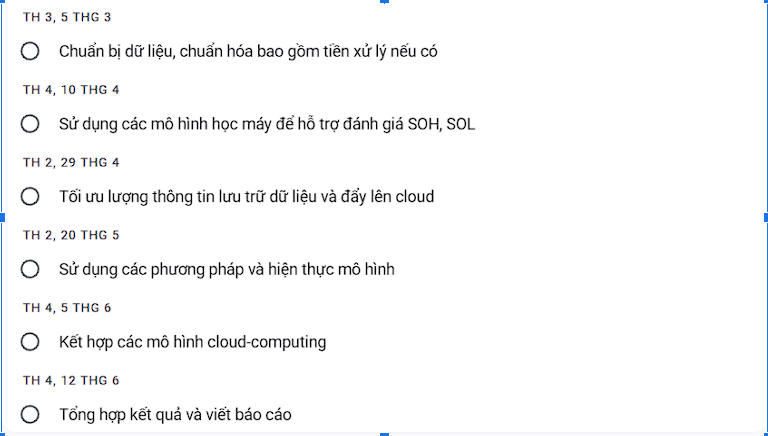
\includegraphics[width=5in]{plan.png}
\end{center}
\end{figure} 

\vspace{5cm}
\section{NỘI DUNG DỰ KIẾN CỦA LUẬN VĂN}

Nội dung báo cáo của luận văn dự kiến sẽ bao gồm các phần như sau:\\

\textbf{Chương 1: Giới thiệu}. Trong chương này sẽ trình bày một số vấn đề cơ bản của đề tài, nêu lên sự quan trọng của việc kiểm tra và giám sát thành phần trong xe điện trong lĩnh vực dữ liệu số hóa. Từ đó thấy được tầm quan trọng của đề tài để xác định rõ phạm vi và đối tượng nghiên cứu, hướng giải quyết của đề tài.
\\

\textbf{Chương 2: Các công trình nghiên cứu liên quan.} Trong chương này sẽ trình bày các công trình nghiên cứu liên quan. Tìm hiểu các phương pháp giải quyết vấn đề cũng như phạm vi, giới hạn của các nghiên cứu đó. Từ đó đánh giá tính khả thi của đề tài.\\

\textbf{Chương 3: Hiện thực và thử nghiệm mô hình. } Trong chương này sẽ trình bày chi tiết cách thức hiện thực của mô hình. Bao gồm các bước xây dựng và huấn luyện mô hình, sử dụng các mô hình và heuristic để giải quyết bài toán.\\

\textbf{Chương 4: Kết quả và đánh giá.} Trong chương này sẽ nêu ra các kết quả đạt được của mô hình, cũng như phương pháp đánh giá các kết quả đó.\\

\textbf{Chương 5: Kết luận.} Trong chương này sẽ tóm lại các ưu điểm và nhược điểm của mô hình và đưa ra các hướng nghiên cứu phát triển hệ thống trong tương lai.\\

\section{KẾT LUẬN}
Việc giám sát và quản lý pin đóng vai trò quan trọng trong đảm bảo hiệu suất, tuổi thọ và an toàn của hệ thống pin trên xe điện. Các công trình nghiên cứu liên quan đã tập trung vào các khía cạnh quan trọng như ước lượng trạng thái sạc và sức khỏe pin, chẩn đoán và tiên đoán lỗi, và quản lý thông minh của pin.\\

Để giám sát pin trên xe điện một cách hiệu quả, cần phải có hệ thống quản lý pin (BMS) thông minh và chính xác. BMS sẽ thu thập dữ liệu về trạng thái pin như trạng thái sạc, nhiệt độ, điện áp và dòng điện, sau đó phân tích và đưa ra các quyết định để bảo vệ pin và tối ưu hóa hiệu suất sử dụng năng lượng.\\

Công nghệ và phương pháp giám sát pin ngày càng phát triển, bao gồm sự kết hợp của cảm biến, hệ thống ghi dữ liệu, trí tuệ nhân tạo và học máy. Các phương pháp này giúp ước lượng trạng thái sạc và sức khỏe pin một cách chính xác, phát hiện và chẩn đoán lỗi một cách nhanh chóng, và dự đoán tuổi thọ còn lại của pin.\\

Thông qua việc nghiên cứu và áp dụng các công trình liên quan, có thể nâng cao hiệu suất và tuổi thọ của pin trên xe điện, giúp tăng khả năng di chuyển và đáp ứng nhu cầu của người sử dụng. Đồng thời, việc giám sát pin cũng đóng vai trò quan trọng trong việc đảm bảo an toàn và hạn chế các vấn đề liên quan đến pin như quá nhiệt, quá điện áp hoặc quá dòng điện.\\

Tổng quan, đề tài "Giám sát pin trên xe điện" là một lĩnh vực nghiên cứu quan trọng và đầy triển vọng, đóng góp vào sự phát triển của công nghệ pin và xe điện hiệu quả và bền vững.\\

\begin{thebibliography}{19}
    \bibitem
    [As87] Astrahan, M.M., Schkolnick, M., Whang, K.-Y. (1987)
    “Approximating the number of unique values of an attribute without
    sorting”, Journal Information Systems, Vol. 12 (1), pp. 11-15,
    Oxford, UK.
    
    \bibitem[Du03] Durand, M., Flajolet, P. (2003) “Loglog Counting of Large
    Cardinalities (Extended Abstract)”, In: G. Di Battista and U.
    Zwick (Eds.) - ESA 2003. Lecture Notes in Computer Science, Vol.
    2832, pp. 605-617, Springer, Heidelberg.
    
    \bibitem[Fl85] Flajolet, P., Martin, G.N. (1985) “Probabilistic Counting
    Algorithms for Data Base Applications”, Journal of Computer and
    System Sciences, Vol. 31 (2), pp. 182-209.
    
    \bibitem[Fl07] Flajolet, P., et al. (2007) “HyperLogLog: the analysis of a nearoptimal cardinality estimation algorithm”, Proceedings of the 2007
    International Conference on Analysis of Algorithms, Juan les Pins,
    France - June 17-22, 2007, pp. 127-146.
    
    \bibitem[He13] Heule, S., et al. (2013) “HyperLogLog in Practice: Algorithmic
    Engineering of a State of The Art Cardinality Estimation Algorithm”, Proceedings of the 16th International Conference on Extending
    Database Technology, Genoa, Italy —- March 18-22, 2013, pp. 683-
    692, ACM New York, NY.
    
    \bibitem[Sc07] Scheuermann, B., Mauve, M. (2007) “Near-optimal compression
    of probabilistic counting sketches for networking applications”,
    Proceedings of the 4th ACM SIGACT-SIGOPS International
    Workshop on Foundation of Mobile Computing (DIAL M-POMC),
    Portland, Oregon, USA. - August 16, 2007.
    
    \bibitem[Wh90] Whang, K.-Y., Vander-Zanden, B.T., Taylor H.M. (1990)
    “A Linear-Time Probabilistic Counting Algorithm for Database
    Applications”, Journal ACM Transactions on Database Systems,
    Vol. 15 (2), pp. 208-229.
\end{thebibliography}
\end{document}